\documentclass[11pt]{article}
%第二十届中国研究生数学建模竞赛论文模板
\usepackage{graphicx,float}%使用图的宏包,使用图的浮动体宏包,引入参数H使图像紧跟当前文字
\usepackage{caption} %使用图表标题的宏包
\usepackage[colorlinks=true,pdfstartview=FitH,%
linkcolor=black,anchorcolor=violet,citecolor=magenta]{hyperref}%加载hyperref宏包,使用超链接
\usepackage{setspace}%用于设置行间距列间距等命令的宏包
\usepackage{array}%设置列表高度宽度的宏包
\usepackage{zhnumber}%使用中文数字编号的宏包
\usepackage{titlesec,titletoc}%使用标题自定义形式的宏包和使用目录自定义形式的宏包
\usepackage{siunitx}%物理学单位宏包
\usepackage{tabularx}%让表格宽度等于页面宽度
\usepackage{makecell}%单个表格单元调整的宏包
\usepackage{booktabs}%给表格添加框线的命令
\usepackage{subfigure} %%使用子图的宏包
\usepackage[backend=biber,bibstyle=gb7714-1987,%nature,%%加载biblatex宏包,使用参考文献
citestyle=gb7714-1987%,backref=true%%其中后端backend使用biber
,url=false
]{biblatex}%标注(引用)样式citestyle,著录样式bibstyle都采用gb7714-2015样式
% \usepackage{pgfplots}%类似tikz的一个画图库,主要画统计图
\usepackage{customFont}%自行编写的字体命令库,基于CJK宏包
\usepackage{customFormat}%自行编写的风格文件,基于使用习惯和格式要求
\usepackage{customMath}%自行编写的数学公式命令库,基于amsmath宏包
\usepackage{customPicture}%集成图形绘制库,主要包括了tikz和pgfplots两大主流宏包
% \usepackage[lite,subscriptcorrection,slantedGreek,nofontinfo]{mtpro2}%使用mathtimepro2商业字体作为数学环境,并不推荐

%biblatex宏包的参考文献数据源加载方式,注意book.bib应当与.tex文件在同一目录下,不然有可能会报错
\addbibresource[location=local]{reference.bib}
% % \bibliographystyle{gbt7714-numerical}
%%% 下面的命令重定义页面边距,使其符合中文刊物习惯 %%%%
% \addtolength{\topmargin}{2.5cm}
\setlength{\oddsidemargin}{0.63cm}  % 3.17cm - 1 inch
\setlength{\evensidemargin}{\oddsidemargin}
% \setlength{\textwidth}{14.66cm}
% \setlength{\textheight}{24.00cm}    % 24.62

\graphicspath{{./fig}}
\begin{document}
\begin{center}

  \begin{figure}[H]
    
\includegraphics[width=0.2\textwidth]{标题图1.png}
    \hspace{0mm}
    
\includegraphics[width=0.2\textwidth]{标题图2.png}
    \hspace{3mm}
    
\includegraphics[width=0.14\textwidth]{标题图3.png}
    \hspace{4mm}
    
\includegraphics[width=0.16\textwidth]{标题图4.png}
    \hspace{4mm}
    
\includegraphics[width=0.18\textwidth]{标题图5.png}
  \end{figure}
  \large{\xiaoerhao\hwxw{\textbf{中国研究生创新实践系列大赛}}}\\
  \large{\erhao\hwxw{\textbf{“华为杯”第二十届中国研究生}}}\\
  \large{\erhao\hwxw{\textbf{数学建模竞d赛}}}
  \vspace{8em}

  \begin{spacing}{2.0}
    \begin{tabular}{m{0.2\textwidth}<{\centering}m{0.6\textwidth}<{\centering}}
      {\xiaoerhao\hwzs{学\quad \quad 校}} & {\xiaoerhao\hwzs{北京航空航天大学}}                                                 \\
      \cmidrule(r){1-2}
      {\xiaoerhao\hwzs{参赛队号} }          & {\xiaoerhao\hwzs{23100060015} }                                             \\
      \cmidrule(r){1-2}
      {\xiaoerhao\hwzs{队员姓名}}           & \begin{tabular}{m{0.1\textwidth}<{\centering}m{0.45\textwidth}<{\centering}}
                                            \xiaoerhao{1.} & \xiaoerhao\hwzs{葛瑄}  \\    \cmidrule(r){1-2}
                                            \xiaoerhao{2.} & \xiaoerhao\hwzs{张严}  \\    \cmidrule(r){1-2}
                                            \xiaoerhao{3.} & \xiaoerhao\hwzs{陈博非} \\
                                          \end{tabular}
      \\
      \bottomrule
    \end{tabular}

  \end{spacing}
\end{center}
\thispagestyle{empty}
\newpage

\begin{center}
  \large{\xiaoerhao\hwxw{\textbf{中国研究生创新实践系列大赛}}}\\
  \large{\erhao\hwxw{\textbf{“华为杯”第二十届中国研究生}}}\\
  \large{\erhao\hwxw{\textbf{数学建模竞赛}}}
  \vspace{2em}
  \par
\end{center}
\begin{table}
  \renewcommand{\arraystretch}{2}
  \begin{tabular}{m{0.2\textwidth}<{\centering}m{0.6\textwidth}<{\centering}}
    \xiaoerhao\lishu{ 题\quad\quad 目:} & \dlmu{\xiaoerhao\lishu{B题:含正则项的梯度下降}}   \\
                                      & \dlmu{\xiaoerhao\lishu{和遗传算法修正的矩阵分解拟合}} \\
  \end{tabular}
\end{table}
\begin{abstract}
  本文结合了线性空间的一般性结论和最优化理论,使用矩阵函数的梯度优化对该函数的最小值估计,得到对离散傅里叶变换矩阵(Discrete Fourier Transform,缩写为DFT)的连续空间最优估计,估计得到的矩阵在平方平均(Frobenius范数)意义下取得最小值。针对离散情况下的估计要求,本文利用连续空间最优估计得到的候选矩阵序列,使用遗传算法在带有约束条件下进一步逼近离散傅里叶变换矩阵真值,在DFT矩阵为4阶的时候,将其分解为3个矩阵的乘积取得了最小方均根误差为$2.27\times10^{-4}$的结果。本文从实践上验证了,在多种学习率、阶数和分解序列个数的情况下,将较低维度(16维以下)的DFT矩阵分解为3至4个矩阵即可取得较好的逼近效果,最小方均根误差平均为0.2,硬件复杂度在4维矩阵情况下可低至22,在8维的情况下可低至158。本文取得的将对应的DFT矩阵按给定误差要求进行分解,这部分分解表格将在附录部分列出。
\end{abstract}
{\xiaoerhao\lishu 关键词:梯度下降法,遗传算法,正则项}
%目录
\newpage
\linespread{1.5}
\setcounter{tocdepth}{3}
%设定目录深度                      
\tableofcontents
%列出目录
\newpage
\linespread{1}
\begin{section}{背景与问题重述}
 \begin{subsection}{问题背景}
   离散傅里叶变换,是傅里叶变换在时域和频域上都呈离散的形式,将信号的时域采样变换为其DTFT的频域采样。在形式上,变换两端(时域和频域上)的序列是有限长的,而实际上这两组序列都应当被认为是离散周期信号的主值序列。即使对有限长的离散信号作DFT,也应当将其看作其周期延拓的变换。在实际应用中通常采用快速傅里叶变换计算DFT。
   \par
   快速傅里叶变换(Fast Fourier Transform, FFT),是快速计算序列的离散傅里叶变换(DFT)或其逆变换的算法\cite{cooley_algorithm_nodate},是一种基于软件设计的傅里叶变换加速方法。傅里叶分析将信号从原始域(通常是时间或空间)转换到频域的表示或者逆过来转换。FFT会通过把DFT矩阵分解为稀疏(大多为零)因子之积来快速计算此类变换。因此,它能够将计算DFT的复杂度从只用DFT定义计算需要的$O(n^2)$,降低到$O(n\log n)$,其中$n$为数据大小。
   令$x_0,x_1,\cdots,x_{N-1}$为复数,DFT由以下式子定义:
   \begin{equation}
     X(k)=\sum_{n=0}^{N-1}x_n\mathrm{e}^{-\mathrm{i}2\pi kn/N},k=0,1,\cdots,N-1
   \end{equation}
   \par
   直接按这个定义求值需要$O(N^2)$次运算: $x_k$共有$N$个输出,每个输出需要有$N$项求和,直接使用DFT运算需使用$N$个复数乘法($4N$个实数乘法)与$N-1$个复数加法($2N-2$个实数加法),因此,计算使用DFT所有$N$点的值需要$N^2$复数乘法与$N^2-N$个复数加法。FFT则是能够在$O(N\log N)$次操作计算出相同结果的方法。
   \par
   DFT的蝶形运算思想是一种分治法的思想,通过不断地分解和合并数据来计算DFT,相对于直接DFT矩阵乘积的形式大幅度降低了复数乘法运算的次数。DFT也可以通过矩阵连乘拟合近似获得,其核心思想是将DFT矩阵近似表达为一连串稀疏的、元素取值有限的矩阵连乘形式。
 \end{subsection}
 \begin{subsection}{问题重述}
   本题目是在硬件复杂度的基础上,根据硬件需求设计软件,优化离散傅里叶变换的计算过程,使得计算过程的复杂度最小,即计算过程中的乘法器个数最少。除了经典的快速傅立叶变换算法从软件上优化计算过程,提高运算速度;还可以从硬件上出发,通过改进矩阵乘法过程,使其实现尽可能少的乘法、甚至是复数乘法。在较低的信号质量需求下,使用硬件改进设计加速离散傅里叶变换能够获得更简洁的硬件设计、更快的执行速度的更低的功率能耗等优势。
   \par
   \begin{itemize}
     \item 问题一要求尽可能增加分解矩阵的零元素,使分解的矩阵序列每行非零元素至多2次,即尽可能稀疏,稀疏的矩阵在计算过程中可以极大地减少乘法次数、即减少乘法器数目。该问题建立在连续的矩阵空间中,因此可以利用连续性和可导性,使用梯度下降法求解最优解;
     \item 问题二、问题三、问题四和问题五与问题一采取了不同的硬件优化手段,即通过限制矩阵元素位数,保证矩阵中各个元素的实部虚部都是2的整 数幂,从而将乘法运算简化为移位运算,从原理上进一步提高计算速度。问题二、问题三 在离散空间中进行矩阵分解,问题四提出了一种新的思维方式,即能否通过已知的低维矩阵的分块、组合,求解高维矩阵的连乘分解。问题五则是对硬件优化过程中提出了更加量化的指标,即限制拟合方均根误差(RMSE)的大小,从而使得拟合结果更加接近真实值,对矩阵分解提出了更高的要求。
   \end{itemize}
 \end{subsection}
\end{section}
\begin{section}{假设与前提}
 \begin{subsection}{基本假设}
   \begin{itemize}
     \item[\textbullet] 遗传算法中,每个父代繁殖得到的子代个体,其遗传的参数服从正态分布,该正态分布与父代和环境有关,为了简化问题,仅考虑该分布与父代个体本身有关;
     \item[\textbullet] 遗传算法中,每个父代个体均以自身克隆的方式繁殖,不考虑有性生殖方式;
     \item[\textbullet] 每个子代的变异概率均服从相同的概率分布列,且各个子代的变异概率相互独立;
   \end{itemize}
 \end{subsection}
 \begin{subsection}{符号列表}

   本文使用的符号及其物理含义如下表所示:\\
   \begin{table}[H]
     \centering
     \renewcommand{\arraystretch}{1.5}
     \caption{本文使用符号及物理含义表}
     \begin{tabular}{c|c|c}
       \hline
       符号名       & 符号表示              & 表达含义                                                                                \\
       \hline
       离散傅里叶变换矩阵 & $\mathbf{F}_N$    & $N$是矩阵的阶数                                                                           \\
       分解得到的矩阵个数 & $K$               & --                                                                                  \\
       分解得到的矩阵   & $\mathcal{A}$     & $\mathcal{A}=\{\mathbf{A}_i,i=0,1,\cdots,K\}$                                       \\
       乘法器的个数    & $C$               & 也是矩阵乘法的复杂度                                                                          \\
       矩阵元素      & $\mathbf{A}[l,m]$ & $l,m=1,2,\cdots,N$                                                                  \\
       矩阵元素取值范围  & $q$               & $\mathbf{A}_k[l,m]\in\{x+yj|x,y\in\mathcal{P}=\{0,\pm1,\pm2,\cdots,\pm 2^{q-1}\}\}$ \\
       矩阵的阶数     & $N$               & $N=2^t,t=1,2,\cdots,q-1$                                                            \\
       克罗内克积     & $\otimes$         & 即矩阵的直积                                                                              \\
       学习率       & lr                & 机器学习的学习率                                                                            \\
       遗传算法个体    & $P_{idv}$         & 是一个算子                                                                               \\
       遗传算法个体超参数 & $\alpha$          & 称该参数为个体“量化参数”                                                                       \\
       适应度函数     & $E$               & 表征当前个体拟合结果与真值的均方根                                                                   \\
       \hline
     \end{tabular}
     \label{table:本文使用符号及物理含义表}
   \end{table}

 \end{subsection}
 \begin{subsection}{基本条件}
   本文主要使用到的数学原理为矩阵导数和最优化理论。以下式子推导矩阵导数的一些基本公式,设$\mathbf{X}$是一个$n\times 1$维的复值向量,矩阵$\mathbf{A}$和$\mathbf{B}$都是$n\times n$维的复值矩阵,那么有:
   \begin{equation}
     \label{eq:矩阵导数1}
     \frac{\partial}{\partial \mathbf{X}}\mathrm{tr}(\mathbf{X}^T\mathbf{A}\mathbf{X})=\mathbf{A}^T+\mathbf{A}
   \end{equation}
   \begin{equation}
     \label{eq:矩阵导数2}
     \frac{\partial}{\partial \mathbf{X}}\mathrm{tr}(\mathbf{X}^T\mathbf{A}\mathbf{X}\mathbf{B})=\mathbf{A}^T\mathbf{X}\mathbf{B}^T+\mathbf{A}\mathbf{X}\mathbf{B}
   \end{equation}
   此外,对于矩阵和矩阵求导的类型,本文主要用到的矩阵的迹运算,因此可以推导得到以下含有对矩阵迹求导的公式:
   \begin{equation}
     \label{eq:矩阵导数3}
     \frac{\partial}{\partial \mathbf{A}}\mathrm{tr}(\mathbf{A}\mathbf{B})= \frac{\partial}{\partial \mathbf{A}}\mathrm{tr}(\mathbf{BA})=\mathbf{B}^\mathrm{T}
   \end{equation}
   \begin{equation}
     \label{eq:矩阵导数4}
     \frac{\partial}{\partial \mathbf{A}}\mathrm{tr}(\mathbf{ABC})= \frac{\partial}{\partial \mathbf{A}}\mathrm{tr}(\mathbf{BCA})=\mathbf{C}^\mathrm{T}\mathbf{B}\T
   \end{equation}
   利用以上公式,可以完成对矩阵函数的逐项求导。设某一矩阵函数$f(\mathbf{A}_1,\mathbf{A}_2,\cdots,\mathbf{A}_r):\mathbb{C}^{n\times n} \longmapsto \mathbb{C}^{n\times n}$,其在连续的复矩阵空间中存在偏导数和梯度,则关于矩阵自变量的梯度可以表示为:
   \begin{align}
     \label{eq:矩阵导数5}
     \nabla f(\mathbf{A}_1,\mathbf{A}_2,\cdots,\mathbf{A}_r)=\rectbrac{\pdiff{f}{\mathbf{A}_1},\pdiff{f}{\mathbf{A}_2},\cdots,\pdiff{f}{\mathbf{A}_r}}\T
   \end{align}
   取定矩阵的微元为:
   \begin{align*}
     \Delta \mathbf{A}=\Delta a\mathbf{I}=\Delta a\left[
       \begin{matrix}
         1      & 0      & \cdots & 0      \\
         0      & 1      & \cdots & 0      \\
         \vdots & \vdots &        & \vdots \\
         0      & 0      & \cdots & 1
       \end{matrix}
       \right],\Delta a=\mathrm{lr}
   \end{align*}
 \end{subsection}

\end{section}
\begin{section}{解题思路及原理}
 \begin{subsection}{梯度下降法}
   对问题一至问题五的复述部分见上,可知各个问题的目标均是使用一个矩阵序列$\{\mathbf{A}_i\}$,对一个已知的矩阵进行逼近,该问题可以转化为矩阵空间上的函数拟合问题,根据题目要求,逼近的判断准则是Frobenius范数即F范数,对以F范数定义的目标函数,将其最小化所得结果如下式:
   \begin{align}
     \min\limits_{\mathcal{A},\beta} \mathrm{RMSE}(\mathcal{A},\beta)=\frac{1}{N}\sqrt{||\beta\mathbf{F}_N-\mathbf{A_1A_2\cdots A}_K||_F^2}\label{eq:目标函数}
   \end{align}
   该函数在整个复矩阵空间内存在全局最小值,将目标函数稍微转换一下形式,对F范数的平方进行处理,平方后的函数与原目标函数具有相同的最小值,即有:
   \begin{align}
     \mathcal{R}(\mathcal{A},\beta)=||\beta\mathbf{F}_N-\mathbf{A_1A_2\cdots A}_K||_F^2
   \end{align}
   利用已知的矩阵求导公式,对函数$\mathcal{R}(\mathcal{A},\beta)$求导,可得:
   \begin{equation}
     \begin{aligned}
       \pdiff{\mathcal{R}}{\mathbf{A}_i} & =\frac{\mathrm{br}(\beta\mathbf{F}_N-\mathbf{A_1A_2\cdots A}_K)\T(\beta\mathbf{F}_N-\mathbf{A_1A_2\cdots A}_K)}{\mathbf{A}_i}                                                                                         \\
                                         & =-2\circbrac{\beta\mathbf{F}_N\mathbf{A}_1\cdots\mathbf{A}_{i-1}\mathbf{A}_{i+1}\cdots\mathbf{A}_K+2\mathbf{A}_i\mathbf{A}_{i+1}\cdots\mathbf{A}_K\mathbf{A}_K^T\cdots\mathbf{A}_{i+1}^T\mathbf{A}_i^T\mathbf{F}_N^T}
     \end{aligned}
     \label{eq:目标函数求导A}
   \end{equation}
   该目标函数除了对矩阵连乘积因子求导外,还需要对系数$\beta$求导,利用公式\ref{eq:矩阵导数4},\ref{eq:矩阵导数5}对系数$\beta$求导可得:
   \begin{equation}
     \begin{aligned}
       \pdiff{\mathcal{R}}{\beta} & =\frac{\mathrm{tr}(\beta\mathbf{F}_N-\mathbf{A_1A_2\cdots A}_K)\T(\beta\mathbf{F}_N-\mathbf{A}_1\mathbf{A}_2\cdots \mathbf{A}_K)}{\beta} \\
                                  & =2\circbrac{\beta\mathbf{F}_N-\mathbf{A}_1\mathbf{A}_2\cdots \mathbf{A}_K}\mathbf{F}_N
     \end{aligned}
     \label{eq:目标函数求导beta}
   \end{equation}
   \par
   利用梯度下降法,对目标函数进行优化,即可得到最优解。梯度下降法的迭代公式为:
   \begin{align}
     \left\{
     \begin{aligned}
       \mathbf{A}_i^{(k+1)} & =\mathbf{A}_i^{(k)}-\Delta\mathbf{A}_i\pdiff{\mathcal{R}}{\mathbf{A}_i}=\mathbf{A}_i^{(k)}-\mathrm{lr}\pdiff{\mathcal{R}}{\mathbf{A}_i} \\
       \beta^{(k+1)}        & =\beta^{(k)}-\Delta\beta\pdiff{\mathcal{R}}{\beta}=\beta^{(k)}-\mathrm{lr}\pdiff{\mathcal{R}}{\beta}
     \end{aligned}
     \right.
     \label{eq:梯度下降法}
   \end{align}
   \par
   理论上,对于任何存在全局最小值的函数,梯度下降法都可以收敛到全局最小值,但是在实际应用中,梯度下降法的收敛速度往往较慢,因此需要对梯度下降法进行改进,本文采用的是Adam算法,其迭代公式为:
   \begin{align}
     \left\{
     \begin{aligned}
       \mathbf{A}_i^{(k+1)} & =\mathbf{A}_i^{(k)}-\frac{\mathrm{lr}}{\sqrt{\hat{v}_i}+\epsilon}\hat{m}_i  \\
       \beta^{(k+1)}        & =\beta^{(k)}-\frac{\mathrm{lr}}{\sqrt{\hat{v}_\beta}+\epsilon}\hat{m}_\beta
     \end{aligned}
     \right.\label{eq:Adam算法}
   \end{align}
   其中,$\hat{m}_i$和$\hat{m}_\beta$分别为对梯度的一阶矩估计,$\hat{v}_i$和$\hat{v}_\beta$分别为对梯度的二阶矩估计,$\epsilon$为一个很小的数,防止分母为0。Adam算法的具体实现过程如下:
   \begin{align}
     \left\{
     \begin{aligned}
       \hat{m}_i^{(k+1)}     & =\frac{\beta_1\hat{m}_i^{(k)}+(1-\beta_1)\pdiff{\mathcal{R}}{\mathbf{A}_i}}{1-\beta_1^{k+1}}   \\
       \hat{v}_i^{(k+1)}     & =\frac{\beta_2\hat{v}_i^{(k)}+(1-\beta_2)\pdiff{\mathcal{R}}{\mathbf{A}_i}^2}{1-\beta_2^{k+1}} \\
       \hat{m}_\beta^{(k+1)} & =\frac{\beta_1\hat{m}_\beta^{(k)}+(1-\beta_1)\pdiff{\mathcal{R}}{\beta}}{1-\beta_1^{k+1}}      \\
       \hat{v}_\beta^{(k+1)} & =\frac{\beta_2\hat{v}_\beta^{(k)}+(1-\beta_2)\pdiff{\mathcal{R}}{\beta}^2}{1-\beta_2^{k+1}}    \\
     \end{aligned}
     \right.\label{eq:Adam算法具体实现}
   \end{align}
   其中$\beta_1$和$\beta_2$是两个在$(0,1)$范围内的常数,用于调节Adam算法的学习矩估计的权重,在本文的使用中取$\beta_1=0.9,\beta_2=0.999$。
   \par
 \end{subsection}
 使用梯度下降法能够求得某个局部最优解$(\tilde{ \mathcal{A}},\tilde{\beta})$,由于本题目中的目标函数并不一定是凸函数,因此不能保证经过梯度下降法得到的结果是全局最小值,对整个复矩阵空间的遍历时间成本太高,在保证符合题目要求的情况下,可以认为求得的矩阵序列和倍缩因子$(\tilde{ \mathcal{A}},\tilde{\beta})$是候选的最佳拟合值$(\mathcal{A}^*,\beta^*)$。在解决第一题的过程中,为了保证最终计算结果能够符合约束条件1:\textbf{\songti 限定$\mathcal{A}$中每个矩阵$\mathbf{A}_i$的每行至多只有两个非零元素}。既要满足约束条件,又要使矩阵收敛至局部最优解,常规的复矩阵空间已经不方便说明。为了解决这样的问题,定义一个增广复矩阵空间$V=\{(\mathbf{A}_1,\mathbf{A}_2,\cdots,\mathbf{A}_K;\beta)|\mathbf{A}_i\in\mathcal{A},\beta\in\mathbb{C}\}$,在该空间下定义一个范数P,以下为其函数表达式:
 \begin{equation}
   P:||(\tilde{\mathcal{A}}',\tilde{\beta}')-(\tilde{ \mathcal{A}},\tilde{\beta})||^2=\sum_{i=1}^{K}||\tilde{\mathbf{A}}_i-\tilde{\mathbf{A}}_i'||_F^2+\gamma^2||\tilde{\beta}-\tilde{\beta}'||^2
   \label{eq:增广矩阵空间向量距离}
 \end{equation}\par
 将上述向量简记为:
 \begin{equation}
   (\mathbf{A}_1,\mathbf{A}_2,\cdots,\mathbf{A}_K;\beta)\triangleq(\mathcal{A},\beta)
 \end{equation}
 在式\ref{eq:增广矩阵空间向量距离}中,$\gamma$是调节向量$(\mathcal{A},\beta)$中表达内积的$\beta$分量所占的权重因子,是一个正实数。可以证明,该范数是该增广矩阵空间中的一个距离。正性、齐次性显然可见,由于Frobenius范数是矩阵空间中的一个距离, 下证定义在V空间中的范数P满足三角不等式:
 \begin{align}
   \begin{aligned}
     ||(\mathcal{A}_1,\beta_1)-(\mathcal{A}_2,\beta_2)||^2 & =\sum_{i=1}^{K}||\mathbf{A}_{1i}-\mathbf{A}_{2i}||_F^2+\gamma^2||\beta_1-\beta_2||^2                                                                                              \\
                                                           & =\sum_{i=1}^{K}||(\mathbf{A}_{1i}\mathbf{A}_{3i})-(\mathbf{A}_{2i}-\mathbf{A}_{3i})||_F^2+\gamma^2||(\beta_1-\beta_3)-(\beta_2-\beta_3)||^2                                       \\
                                                           & \le\sum_{i=1}^{K}||(\mathbf{A}_{1i}\mathbf{A}_{3i})||_F^2+\gamma^2||(\beta_1-\beta_3)||^2+\sum_{i=1}^{K}||(\mathbf{A}_{2i}-\mathbf{A}_{3i})||_F^2+\gamma^2||(\beta_2-\beta_3)||^2 \\
                                                           & =||(\mathcal{A}_1,\beta_1)-(\mathcal{A}_3,\beta_3)||^2+||(\mathcal{A}_2,\beta_2)-(\mathcal{A}_3,\beta_3)||^2
   \end{aligned}
   \label{prof:证明范数P是一个距离}
 \end{align}\par
 因此范数P满足空间距离的三个性质,它是空间V中的一个距离。利用该范数是距离的性质,可以进一步证明\cite{__2012},空间V是稠密的赋范线性空间,因此可以给定任意正数$\epsilon$,必定能够存在一个$\delta,\delta>0$,在这个局部最优解的领域$Q[(\mathcal{A},\beta),\delta]$内找到一个符合条件1的近似最优解$(\tilde{\mathcal{A}}',\tilde{\beta}')$,使之满足:
 \begin{equation}
   ||(\tilde{\mathcal{A}}',\tilde{\beta}')-(\tilde{ \mathcal{A}},\tilde{\beta})||^2=\sum_{i=1}^{K}||\tilde{\mathbf{A}}_i-\tilde{\mathbf{A}}_i'||_F^2+\gamma^2||\tilde{\beta}-\tilde{\beta}'||^2<\epsilon
   \label{eq:稠密性保证矩阵存在最优解的近似解}
 \end{equation}\par
 对于某一个约束条件$\mathcal{D}$,将其引入至迭代过程中,修改公式\ref{eq:梯度下降法}为:
 \begin{align}
   \left\{
   \begin{aligned}
     \mathbf{A}_i^{(k+1)} & =D_k\circbrac{\mathbf{A}_i^{(k)}-\mathrm{lr}\pdiff{\mathcal{R}}{\mathbf{A}_i}} \\
     \beta^{(k+1)}        & =D_k\circbrac{\beta^{(k)}-\mathrm{lr}\pdiff{\mathcal{R}}{\beta}}
   \end{aligned}
   \right.\label{eq:带约束条件的梯度下降法}
 \end{align}\par
 其中,需要保证函数$\prod_{k=1}^\infty D_k=\mathcal{D}$。以上证明过程是保证在不改变梯度的情况下,直接增加约束条件能够使拟合结果收敛至需要值的理论依据。
 \begin{subsection}{遗传算法}
   从第二题开始,拟合的矩阵从连续取值的复值矩阵变成了离散取值,离散空间中不存在$\nabla$算子所定义的梯度,因此直接使用梯度下降法将不再有效。根据证明公式\ref{prof:证明范数P是一个距离}可知,增广矩阵空间是稠密的在每一个向量点周围,都可以以任意精度的离散向量点进行逼近。因此,可以将带有约束条件2:\textbf{\songti 限定$\mathcal{A}$中每个矩阵$\mathbf{A}_k$满足其每个元素的实部和虚部都是2的整数幂,最高幂次为2}的拟合问题抽象为一个增广矩阵空间最优解领域附近的离散取值优化问题。该优化问题的目标函数将仍然以公式\ref{eq:目标函数}的形式表出,增广矩阵空间中的最优解可以使用梯度下降法求解得到,因此不需要完全从头开始计算,只需要从增广空间最优解的小领域内搜索离散情况下的最优解,该离散最优解的分布特点是集中于增广空间的最优解附近,因此可以使用遗传算法对该结果进一步迭代,能够在保证约束条件的情况下进一步优化拟合结果。详细步骤见下列表达:\par
   第一步,对个体编码,选定每个个体是一个算子$P_{idv}(\alpha)\in\mathcal{P}$,该算子将增广矩阵空间中的向量映射为符合约束条件下的离散空间向量,在第二问中,该算子定义的形式为$\displaystyle P_{idv}(\mathcal{A})=\prod_{i=1}^K \frac{Q(\alpha\cdot\mathbf{A}_i)}{\alpha}$,式中,$Q(\bullet)$函数是一个量化函数,将离散空间中的取值映射为以2的幂次为分段点的台阶,其完整定义为:
   \begin{align}
     Q(x)=\left\{
     \begin{aligned}
       0       & ,      & 0\le x< 2^0       \\
       2^0     & ,      & 2^0\le x< 2^1     \\
       2^1     & ,      & 2^1\le x< 2^2     \\
               & \vdots &                   \\
       2^{i-1} & ,      & 2^{i-1}\le x< 2^i \\
               & \vdots &                   \\
       2^{q-1} & ,      & 2^{q-1}\le x< 2^q \\
     \end{aligned}
     \right.\label{eq:离散量化函数}
   \end{align}\par
   式中的$\alpha$是一个超参数,也是遗传算法需要搜索的优化变量。将函数$Q(\bullet)$其依点作用于矩阵的每一个元素,即可以得到对矩阵$\mathbf{A}_i$进行量化后的离散矩阵。\par
   第二步,设定从父代向子代的繁殖和变异规则:不妨假设每一个个体都自带有一个高斯分布$N(\alpha,\sigma)$,式中的$\alpha$是分布均值,表示该父代个体繁殖得到的子代个体量化参数服从以父代量化参数为均值,父代标准差的正态分布。这里取定每个父代均繁殖产生8个子代。繁殖过程中产生变异,变异会对高斯分布的两个参数都产生作用,对各种变异定义变异概率分布列:
   \begin{table}[H]
     \caption{变异概率分布列}
     \centering
     \begin{tabular}{c|c|c|c|c|c}
       \hline
       变异事件 & $\alpha\leftarrow\alpha/k_\alpha$ & $\alpha\leftarrow\alpha\cdot k_\alpha$ & $\sigma\leftarrow\sigma/ k_\sigma$ & $\sigma\leftarrow\sigma\cdot k_\sigma$ & 无变化  \\
       \hline
       变异概率 & 0.03                              & 0.03                                   & 0.1                                & 0.1                                    & 0.74 \\
       \hline
     \end{tabular}
     \label{table:变异概率分布列}
   \end{table}
   \par
   其中,$k_\alpha$是$\alpha$的倍缩变异因子,$k_\sigma$是$\sigma$的倍缩变异因子,根据经验,取定倍缩因子为$k_\alpha=k_\sigma=1.25$。按照以上变异事件概率分布列,在一个父代个体进行克隆繁殖的过程中对每一个子代进行遍历,决定其是否发生变异。\par
   第三步,设定适应度函数,适应度函数的定义为当前个体经量化函数得到的拟合矩阵值与真实的DFT的均方值\ref{eq:目标函数}:
   \begin{align}
     \mathrm{E}(\mathcal{A},\beta)=-\mathrm{RMSE}^2(\mathcal{A},\beta)
   \end{align}
   根据当前的适应度函数得分,对当前个体进行排序,排除后80\%的个体,视为是正常的自然选择。然后,每隔一个固定时间间隔,调用一次“大过滤器”对当前个体进行大规模淘汰,设定某个适应度的阈值,当某个体适应度得分低于此阈值时,以较大概率将其淘汰,当某个体适应度得分高于此阈值时,以较小概率将其淘汰。\par
   完成以上四步设定后,可以进行遗传算法的迭代,迭代过程中,每隔一定时间间隔,将当前个体的最优解输出,作为当前问题的最优解。在迭代过程中,可以设定一个最大迭代次数,当达到最大迭代次数时,遗传算法停止迭代,输出当前个体的最优解,作为当前问题的最优解。整个过程可以按如下流程图所示:
   \begin{figure}[H]
     \centering
     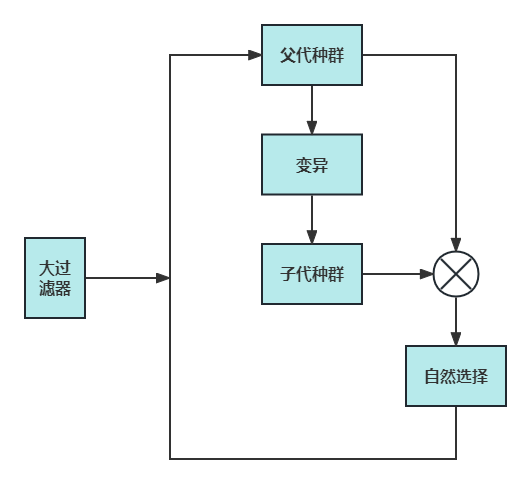
\includegraphics[width=0.6\textwidth]{遗传算法流程.png}
     \caption{遗传算法流程图}
     \label{fig:遗传算法流程图}
   \end{figure}
   \par
   遗传算法将输出在给定约束条件下的离散空间最优解。
 \end{subsection}
\end{section}
\begin{section}{问题解答}
 \begin{subsection}{问题一}
   使用梯度下降法求解矩阵序列,引入正则修正项,若设$max_1{\mathbf{A}}$是当前矩阵$\mathbf{A}$保留各行元素最大值,同时将其他所有值对应位置处置0的函数,根据公式\ref{eq:带约束条件的梯度下降法}的定义,设矩阵中最大的元素组成的矩阵为$\max_1{\mathbf{A}}$,矩阵中第二大的元素组成的矩阵为$\max_1(\mathbf{A}-\max_1\mathbf{A})$,取定正则系数$\lambda,0<\lambda<1$,则可以将正则项函数具体化为:
   \begin{align}
     \lambda(\mathcal{A},\beta)=(1+\lambda)\cdot[\max_1{\mathbf{A}}+\max_1(\mathbf{A}-\max_1\mathbf{A})]+(1-\lambda)\cdot[A-\max_1{\mathbf{A}}-\max_1(\mathbf{A}-\max_1\mathbf{A})]
     \label{eq:正则项函数定义式}
   \end{align}
   \par
   显然,进行$r$次迭代后的正则项函数可以近似表达为:
   \begin{align}
     \lambda(\mathcal{A},\beta) & =(1+\lambda)^r\cdot[\max_1{\mathbf{A}}+\max_1(\mathbf{A}-\max_1\mathbf{A})]        \\
                                & +     (1-\lambda)^r\cdot[A-\max_1{\mathbf{A}}-\max_1(\mathbf{A}-\max_1\mathbf{A})]
     \label{eq:正则项函数多次迭代结果}
   \end{align}
   在不同的情况下,使用梯度下降的过程图,图中横轴表示迭代次数,纵轴表示当前拟合误差:
   \begin{figure}[H]
     \centering
     \subfigure[$lr=1\times 10^{-2}$]{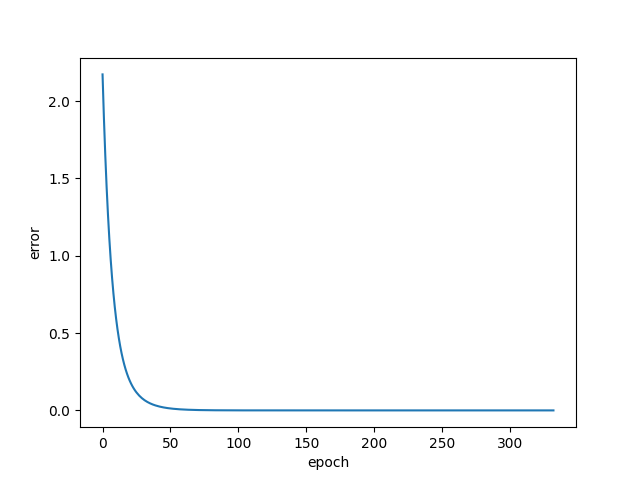
\includegraphics[width=0.4\textwidth]{k=1,t=1,lr=1e-2(epoch-error).png}}
     \subfigure[$lr=1\times 10^{-4}$]{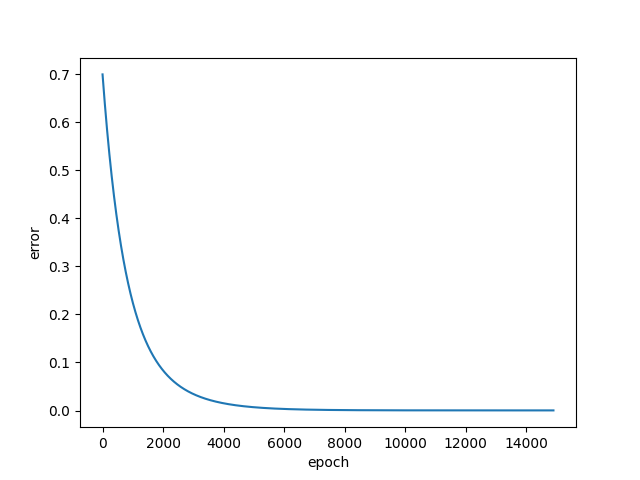
\includegraphics[width=0.4\textwidth]{k=1,t=1,lr=1e-4(epoch-error).png}}
     \subfigure[$lr=5\times 10^{-4}$]{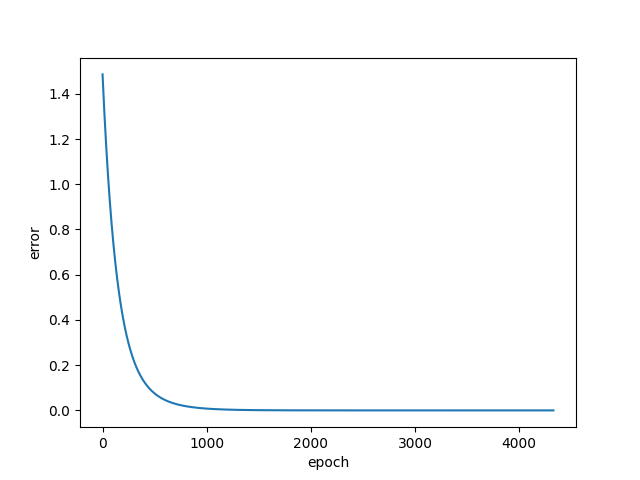
\includegraphics[width=0.4\textwidth]{k=1,t=1,lr=5e-4(epoch-error).png}}
     \subfigure[$lr=8\times 10^{-3}$]{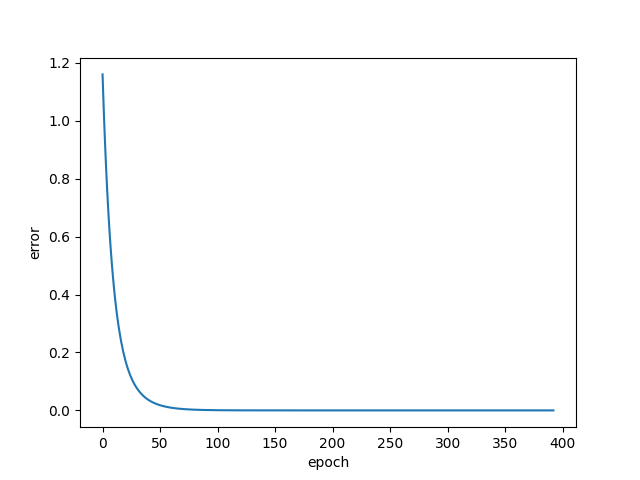
\includegraphics[width=0.4\textwidth]{k=1,t=1,lr=8e-3(epoch-error).png}}
     \label{fig:$K=1,N=2$时梯度下降过程示意图}
     \caption{$K=1,N=2$时梯度下降过程示意图}
   \end{figure}
   由图可知,在矩阵的维数和分解序列的个数都确定的情况下,拟合过程中的计算误差均呈现出随迭代次数增加而减少的趋势,说明基本矩阵梯度的算法能够收敛至某一极小值,且该算法对学习不甚敏感,具有较好的稳健性。同时,在相同条件下,学习率越小,迭代次数越多,最终达到的拟合精度越高。\par
   \begin{figure}[H]
     \centering
     \subfigure[$K=3,lr=1\times 10^{-4}$]{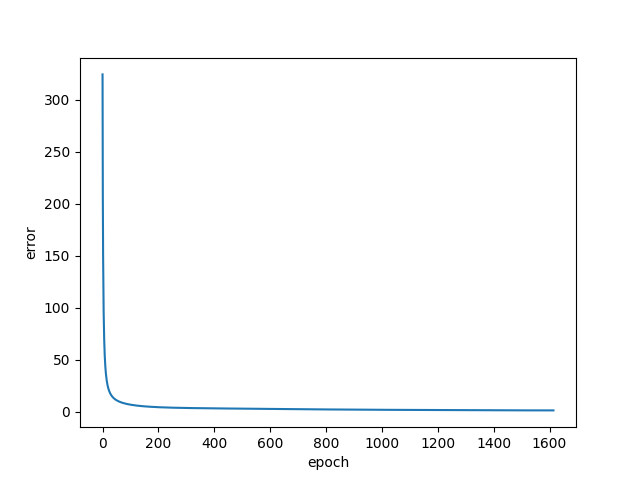
\includegraphics[width=0.3\textwidth]{k=3,t=3,lr=1e-4(epoch-error).png}}
     \subfigure[$K=4,lr=1\times 10^{-5}$]{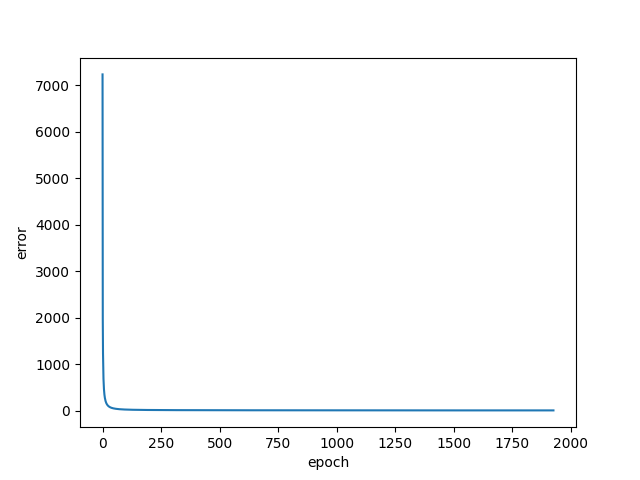
\includegraphics[width=0.3\textwidth]{k=4,t=3,lr=1e-5(epoch-error).png}}
     \subfigure[$K=5,lr=1\times 10^{-5}$]{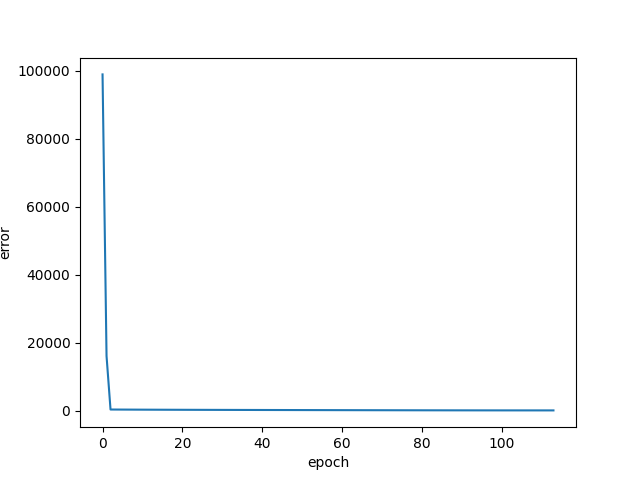
\includegraphics[width=0.3\textwidth]{k=5,t=3,lr=1e-5(epoch-error).png}}
     \label{fig:$t=3$时梯度下降过程示意图}
     \caption{$t=3$时梯度下降过程示意图}
   \end{figure}
   由图可知,在待拟合矩阵的阶数保持固定时,如果增加矩阵分解序列的元素个数,可以较好地提高拟合的精度,同时,分解序列个数增加将会加快梯度下降算法的收敛速度。有关另一个优化参数$\beta$的迭代次数变化曲线如下图所示:\par
   \begin{figure}[H]
     \centering
     \subfigure[$K=3,lr=1\times 10^{-4}$]{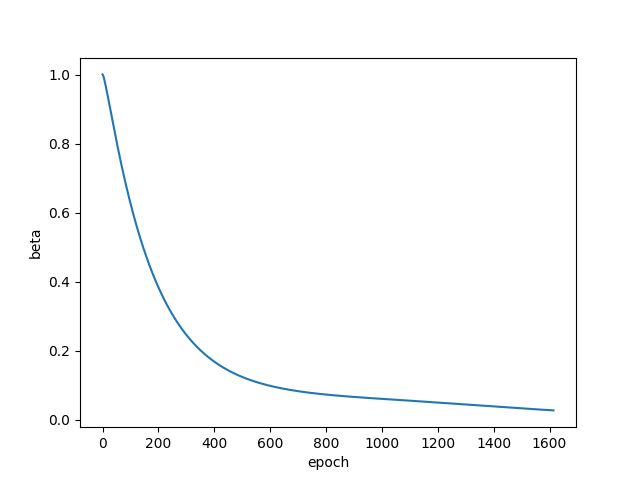
\includegraphics[width=0.3\textwidth]{k=3,t=3,lr=1e-4(epoch-beta).png}}
     \subfigure[$K=4,lr=1\times 10^{-5}$]{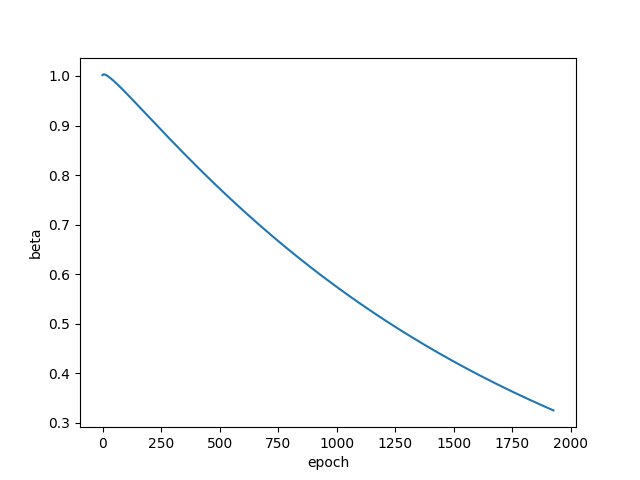
\includegraphics[width=0.3\textwidth]{k=4,t=3,lr=1e-5(epoch-beta).png}}
     \subfigure[$K=5,lr=1e-5$]{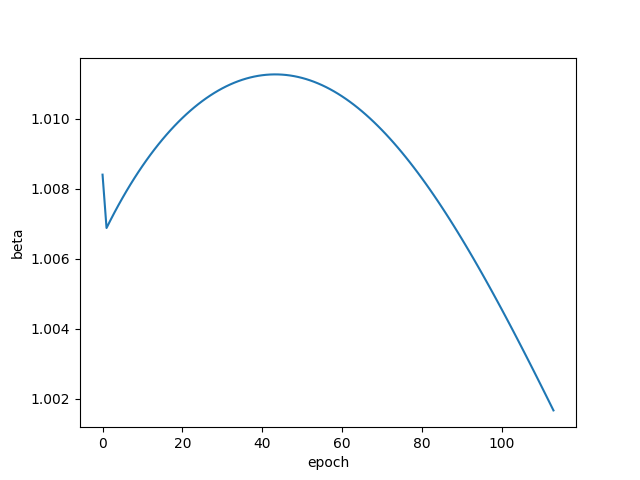
\includegraphics[width=0.3\textwidth]{k=5,t=3,lr=1e-5(epoch-beta).png}}
     \label{fig:$t=3$时梯度下降过程,beta示意图}
     \caption{$t=3$时梯度下降过程,$\beta$示意图}
   \end{figure}
   可见迭代过程中得到的$\beta$值随着迭代次数的进行,$\beta$将逐渐收敛到一个稳定值,这个稳定值与学习率有关,学习率越大,$\beta$收敛的速度越快,最终收敛的值也越大。分解的序列个数越多,取得的误差越小,但是序列数如果过于多,反而增大了$\mathrm{RMSE}$误差。\par
 \end{subsection}
 \begin{subsection}{问题二}
   与问题一的解决方法类似,这里为了使求解得到的分解序列中的矩阵元素都是2的整数幂,需要对矩阵元素进行量化,量化函数的定义见\ref{eq:离散量化函数},在使用遗传算法之前,将连续矩阵空间的最优解比较接近的离散矩阵空间的最优解作为遗传算法的初始值,然后使用遗传算法进行迭代,迭代过程中在解空间中搜索优化个体的$\alpha$值,直到达到一个预期值为止。下图绘制了在同一次迭代过程中,最佳拟合的误差和对应的倍缩因子$\beta$取值情况。
   \begin{figure}[H]
     \graphicspath{{./fig/problem_2}}
     \centering
     \subfigure[$K=3,lr=1\times 10^{-4}$]{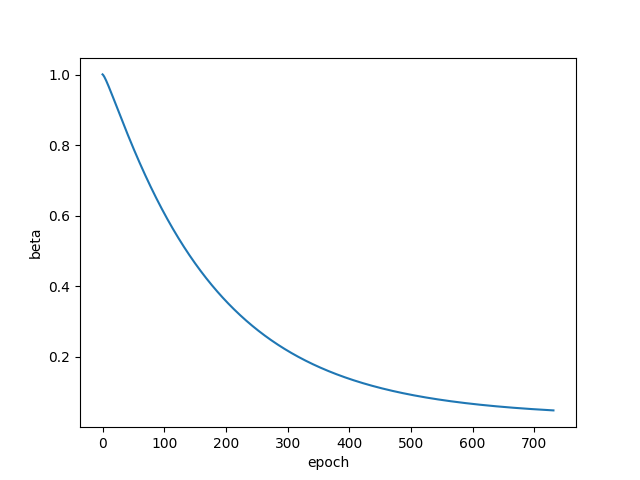
\includegraphics[width=0.4\textwidth]{k=3,t=3,lr=1e-4epoch-beta.png}}
     \subfigure[$K=4,lr=1\times 10^{-5}$]{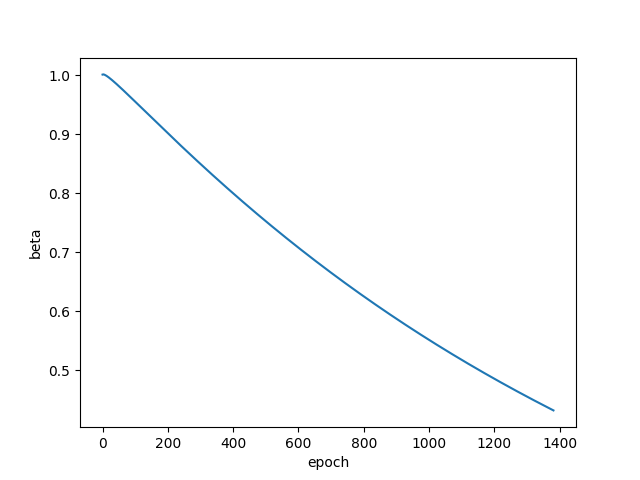
\includegraphics[width=0.4\textwidth]{k=4,t=3,lr=1e-5epoch-beta.png}}
     \subfigure[$K=3,lr=1\times10^{-4}$]{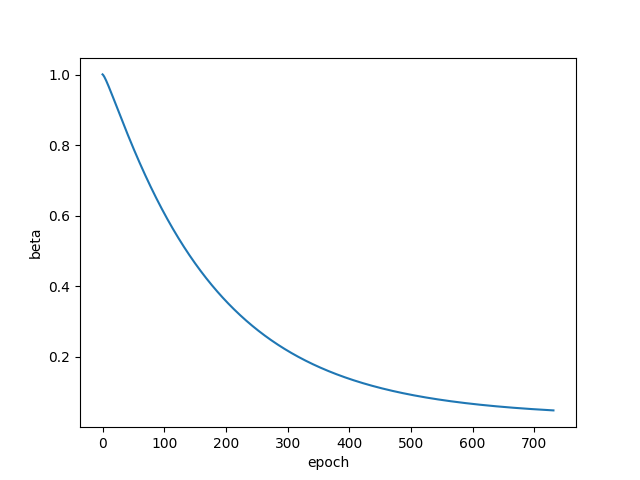
\includegraphics[width=0.4\textwidth]{k=3,t=3,lr=1e-4epoch-beta.png}}
     \subfigure[$K=4,lr=1\times10^{-5}$]{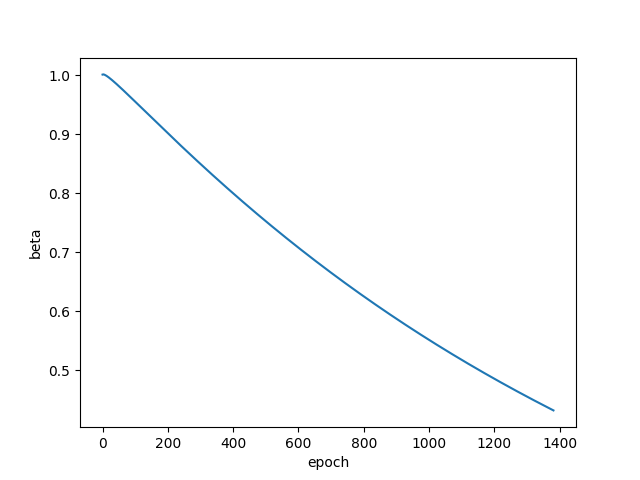
\includegraphics[width=0.4\textwidth]{k=4,t=3,lr=1e-5epoch-beta.png}}
     \label{fig:t=3时遗传算法过程}
     \caption{$t=3$时遗传算法过程示意图}
   \end{figure}
   由图可知,经过遗传算法后,矩阵连乘积结果在离散空间中仍然能够收敛,因此可以在连续空间最优解附近邻域内找到一个近似最优的离散空间解,可以认为该解就是满足\textbf{\songti 约束条件2}的解。随着遗传算法迭代次数增加,拟合误差减少,进一步逼近真值。选用不同的遗传算法迭代次数,得到的拟合误差如下图所示:
   \begin{figure}[H]
     \graphicspath{{./fig/problem_2}}
     \centering
     \subfigure[$N=4,K=3$]{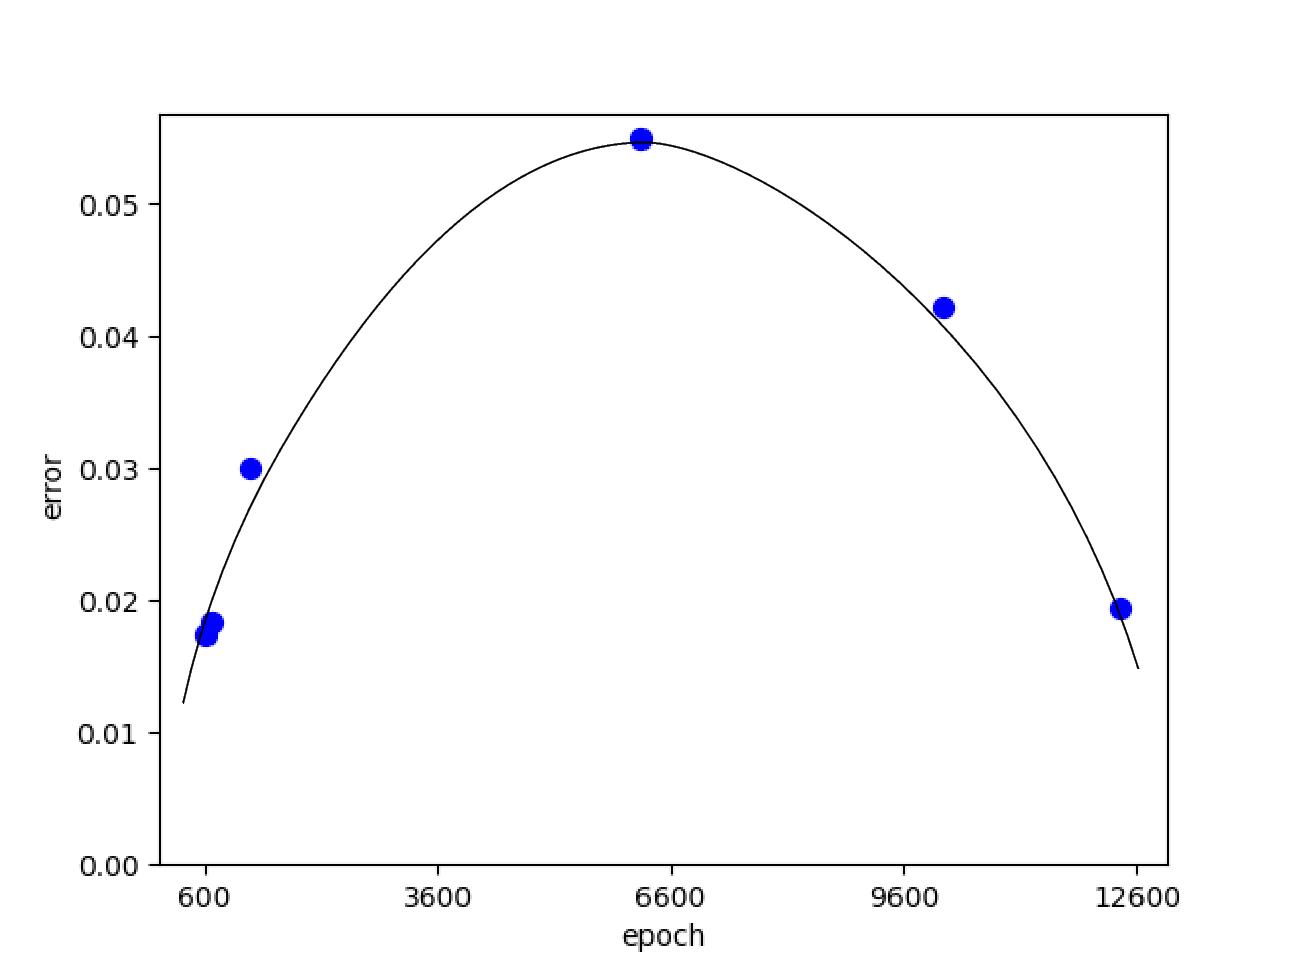
\includegraphics[width=0.4\textwidth]{k=1,epoch-error.jpg}}
     \subfigure[$N=4,K=4$]{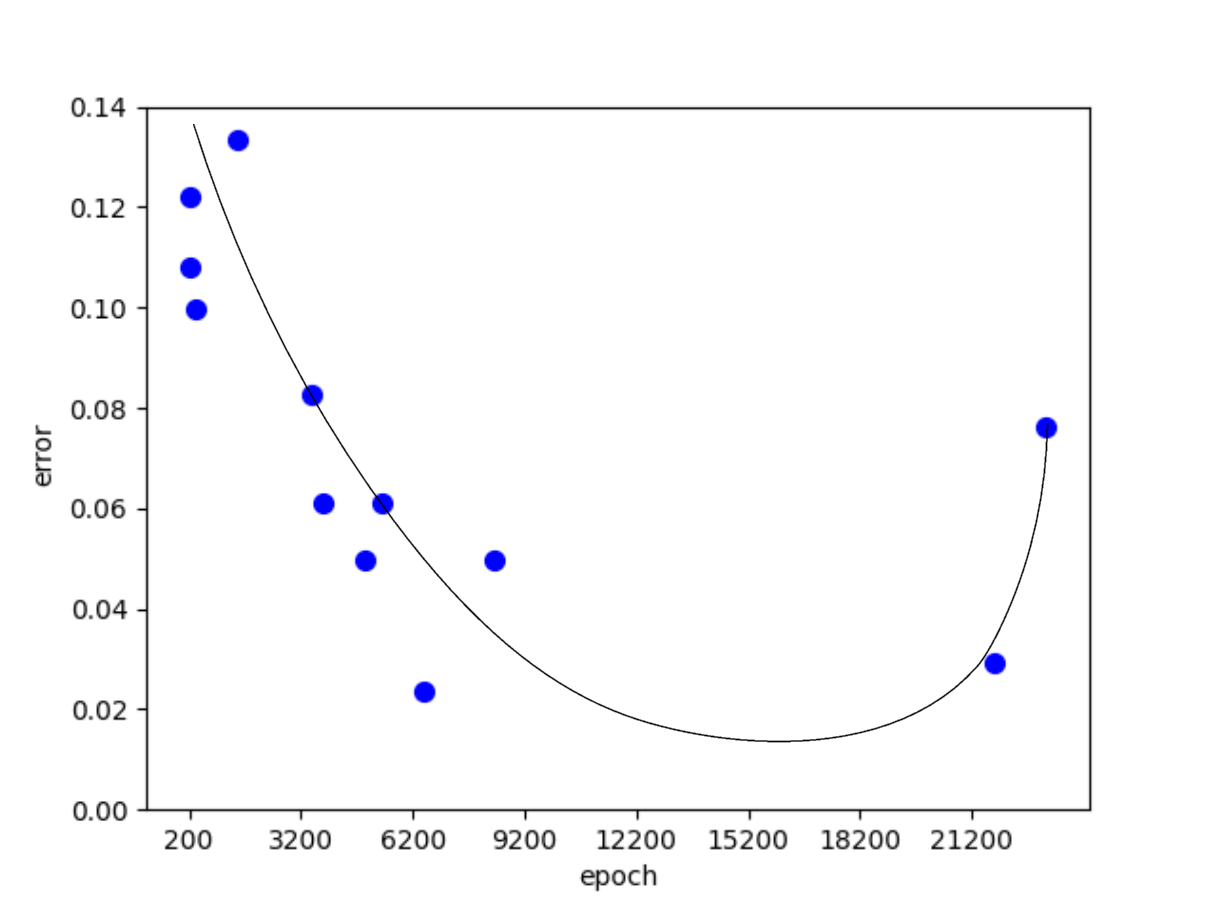
\includegraphics[width=0.4\textwidth]{k=2,epoch-error.jpg}}
     \subfigure[$N=8,K=3$]{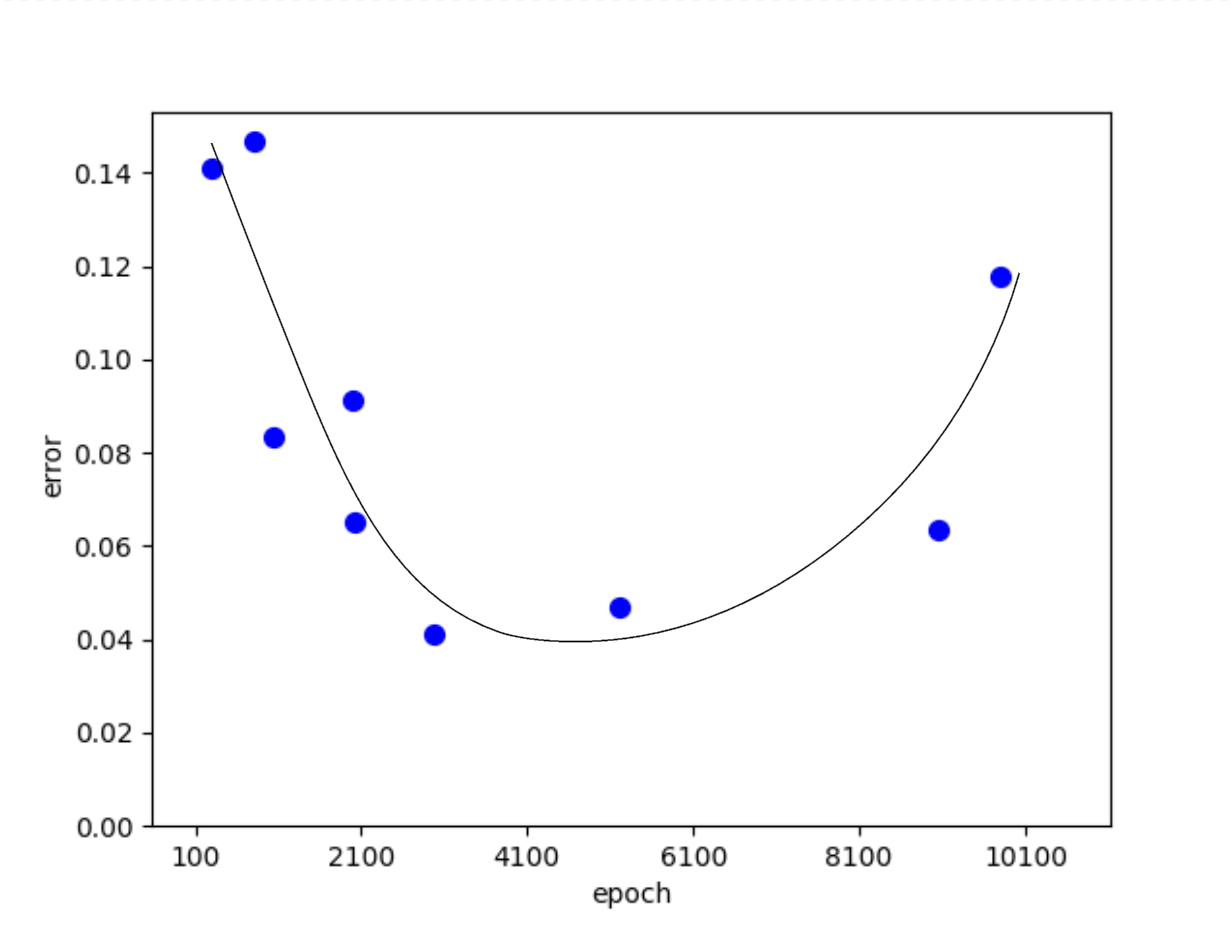
\includegraphics[width=0.4\textwidth]{k=3,epoch-error.png}}
     \subfigure[$N=8,K=4$]{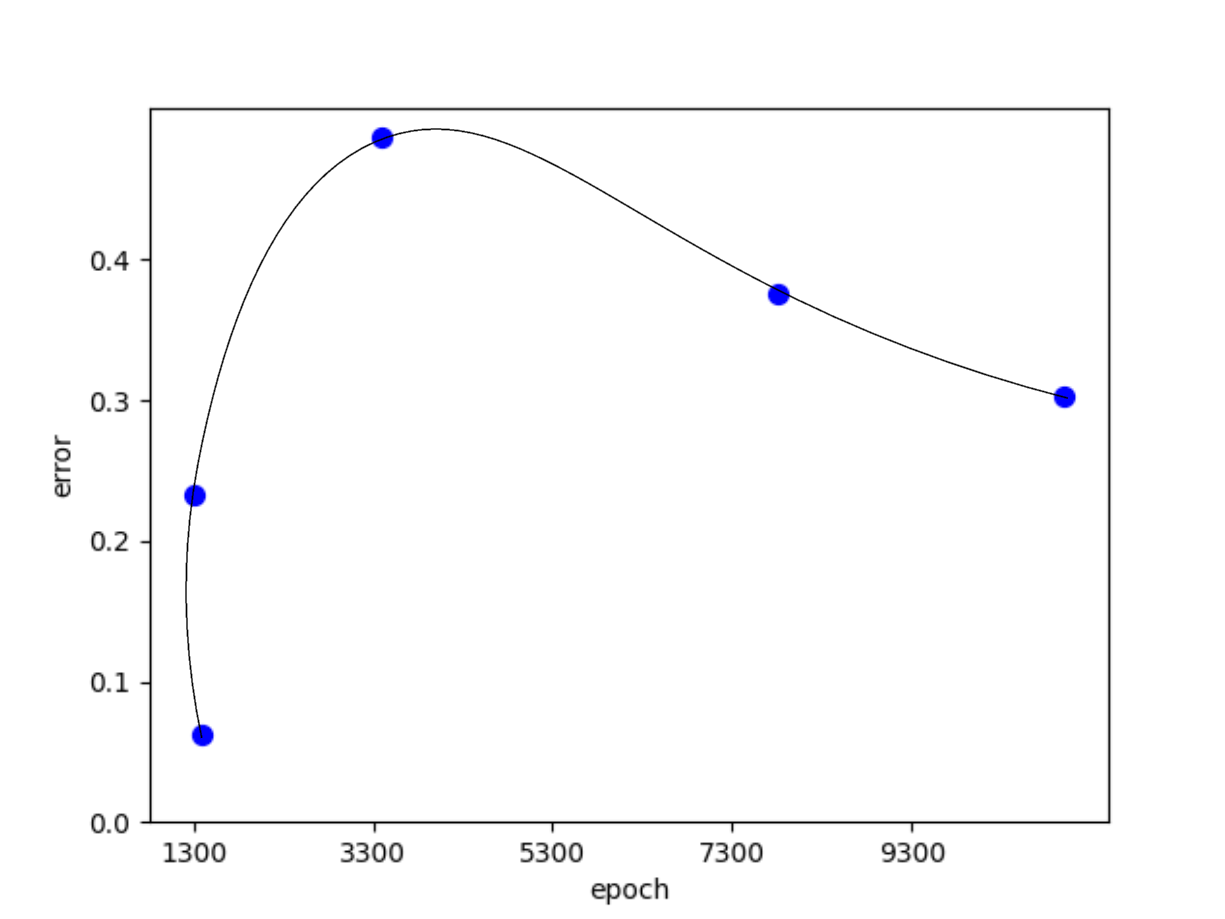
\includegraphics[width=0.4\textwidth]{k=4,epoch-error.jpg}}
     \label{fig:t=3时遗传算法误差与迭代次数的关系}
     \caption{遗传算法误差与迭代次数的关系}
   \end{figure}
   可见,在遗传算法进行过程中,存在一个最小误差,选用合理的迭代次数可能收敛至该最小误差,根据不同情况下的最小误差,使用最佳的迭代次数。
 \end{subsection}
 \begin{subsection}{问题三}
   本问题采取的主要解决思路与问题二是一致的,在问题二的基础上,再次引入公式\ref{eq:正则项函数定义式}所代表的约束条件,与公式\ref{eq:离散量化函数}共同作用于遗传算法的个体,在迭代过程中筛选符合条件的个体,最终得到的结果。
   \begin{figure}[H]
     \graphicspath{{./fig/problem_3}}
     \centering
     \subfigure[$N=4,K=3$]{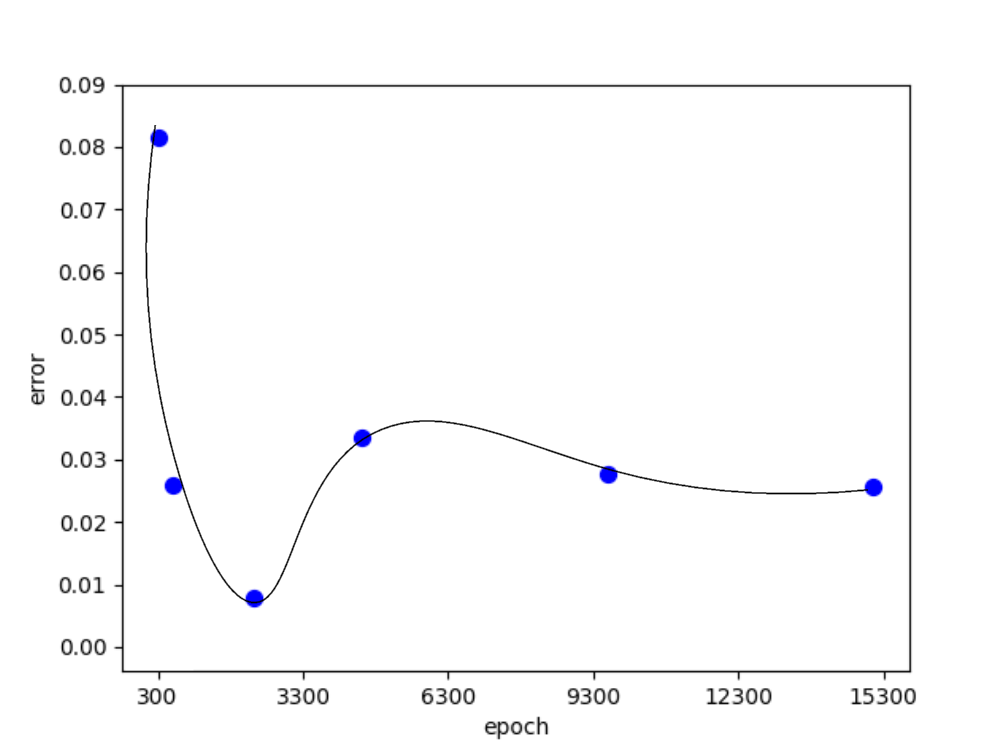
\includegraphics[width=0.4\textwidth]{k=1,epoch-error.jpg}}
     \subfigure[$N=4,K=4$]{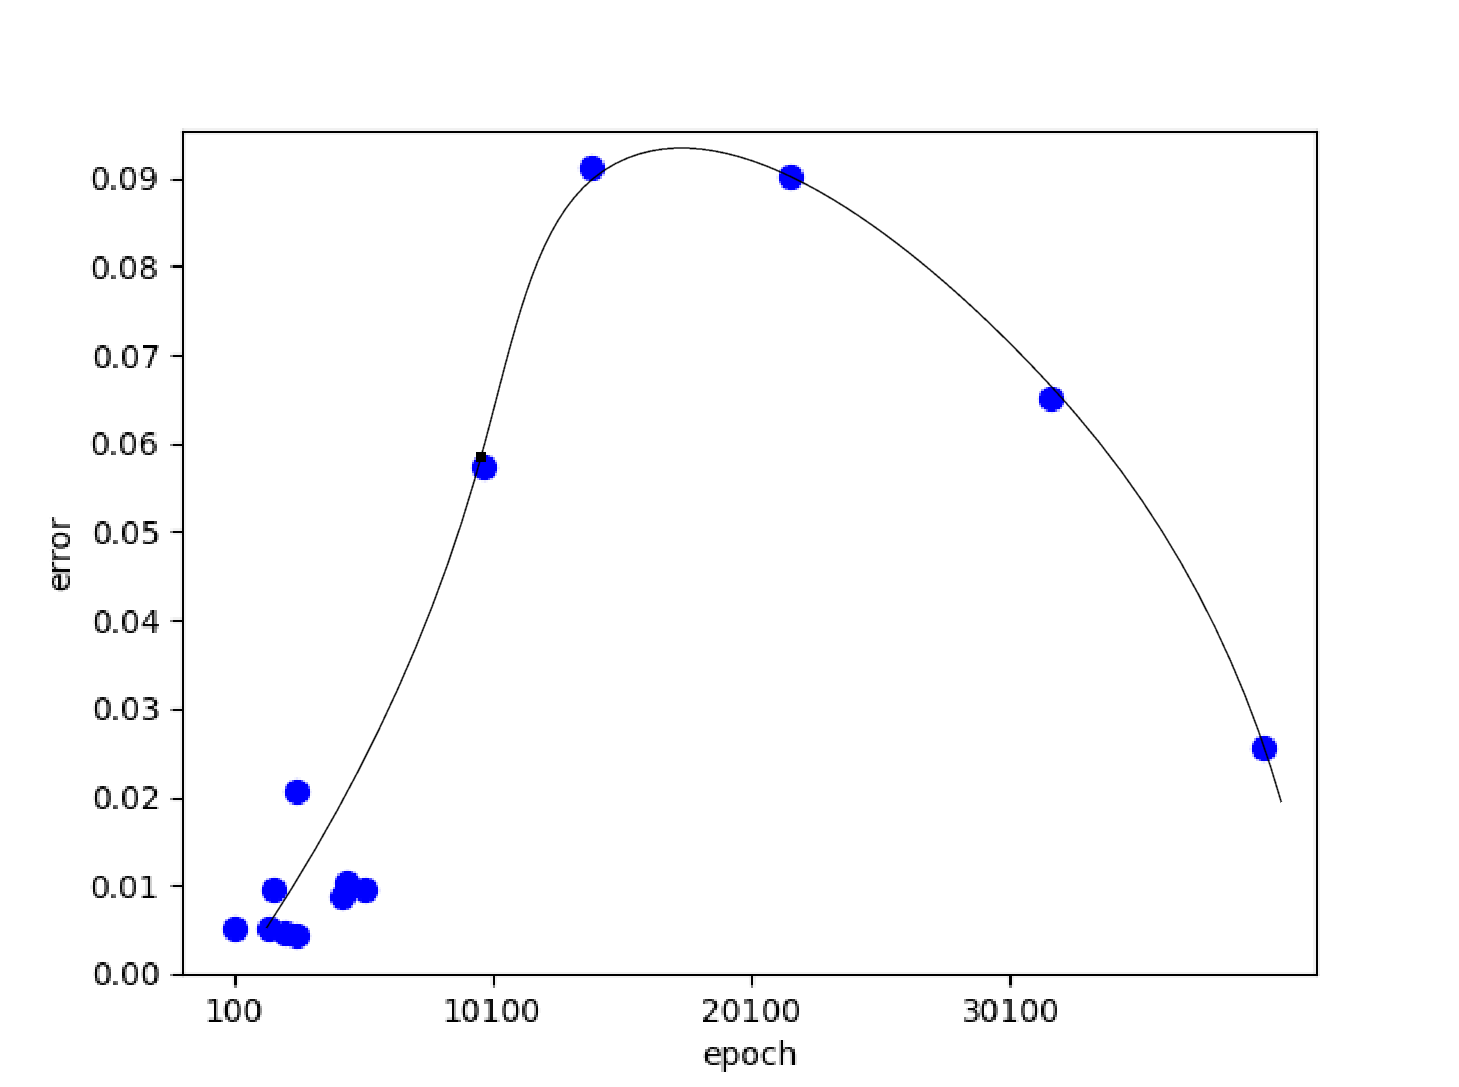
\includegraphics[width=0.4\textwidth]{k=2,epoch-error.jpg}}
     \subfigure[$N=8,K=3$]{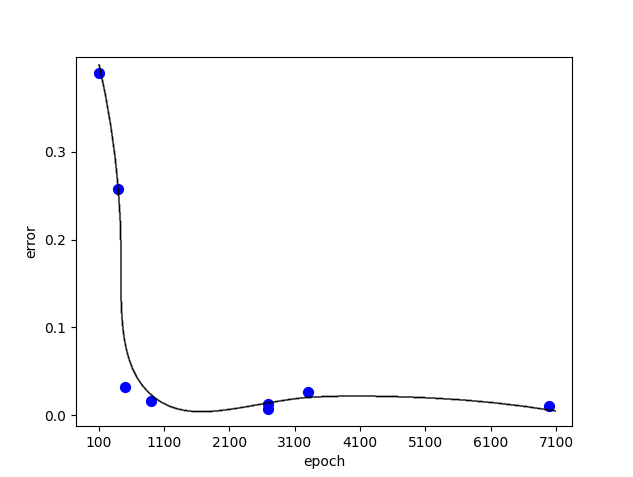
\includegraphics[width=0.4\textwidth]{k=3,epoch-error.jpg}}
     \subfigure[$N=8,K=4$]{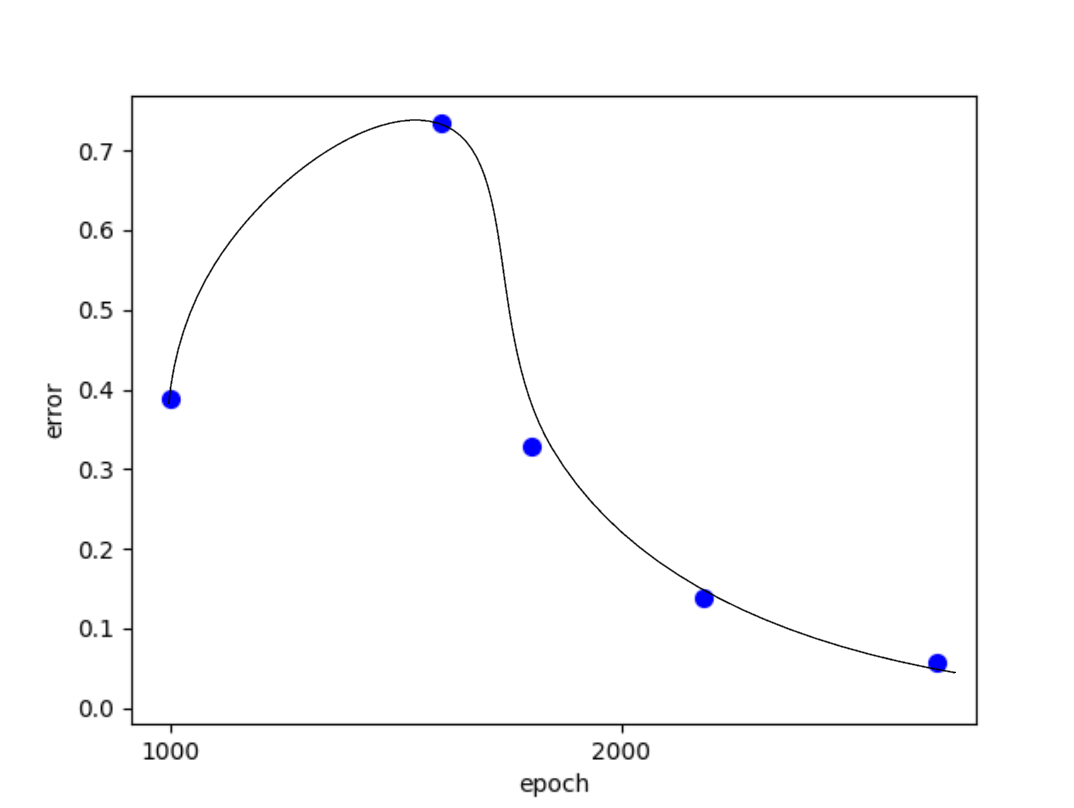
\includegraphics[width=0.4\textwidth]{k=4,epoch-error.jpg}}
     \label{fig:问题三遗传算法误差与迭代次数的关系}
     \caption{遗传算法误差与迭代次数的关系}
   \end{figure}
   由图可知,当前迭代效果因为引入新约束条件而变差。
 \end{subsection}
 \begin{subsection}{问题四}
   虽然矩阵$\mathbf{F}_N$不是DFT 矩阵,但是其可以写成$\mathbf{F}_N=\mathbf{F}_N1⊗\mathbf{F}_N2$的形式,且$\mathbf{F}_N1$ 和$\mathbf{F}_N2$分别是$N_1$和$N_2$维的DFT矩阵。那么根据问题三结论,由于已经把$\mathbf{F}_N1$ 和$\mathbf{F}_N2$分别用若干个元素的实部和虚部受限制的稀疏矩阵的积来拟合,因此,非DFT 矩阵$\mathbf{F}_N$可以用题目三得到的若干个元素实部和虚部受限制的稀疏矩阵的积再做Kronecker积来拟合。同时,对$A$和$\beta$的优化条件保持得和问题三一致即可。在$N_1=4, N_2=8$时,$\mathbf{F}_N1$ 和$\mathbf{F}_N2$分别是4和8维的DFT矩阵。为了得到最优的拟合矩阵,可以取问题三中对4和8维的DFT矩阵进行拟合的矩阵A中最优的,即误差最小的。虽然矩阵$\mathbf{F}_N$不是DFT 矩阵,但是其可以写成$\mathbf{F}_N=\mathbf{F}_N1\otimes \mathbf{F}_N2$的形式,且$\mathbf{F}_N1$ 和$\mathbf{F}_N2$分别是$N_1$和$N_2$维的DFT矩阵。那么根据问题三结论,由于已经把$\mathbf{F}_N1$ 和$\mathbf{F}_N2$分别用若干个元素的实部和虚部受限制的稀疏矩阵的积来拟合,因此,非DFT 矩阵$\mathbf{F}_N$可以用题目三得到的若干个元素实部和虚部受限制的稀疏矩阵的积再做Kronecker积来拟合。同时,对$A$和$\beta$的优化条件保持得和问题三一致即可。在$N_1=4, N_2=8$时,$\mathbf{F}_N1$ 和$\mathbf{F}_N2$分别是4和8维的DFT矩阵。为了得到最优的拟合矩阵,可以取问题三中对4和8维的DFT矩阵进行拟合的矩阵$\mathcal{A}$中最优的,即误差最小的。\par
   通过对实验三的运行结果,可以得到:\par
   对于四阶DFT 矩阵$\mathbf{F}_N$,其最优的情况,即误差最小的情况是用两个四阶元素实部和虚部受限制的稀疏矩阵的积做拟合,(此时取学习率$lr= 1e-5$,参数$\beta=0.3354$,误差$\mathrm{RMSE}=0.09109$),样例矩阵为:
   \begin{align}
     \mathbf{A}_1=\left[
       \begin{matrix}
         0    & 4-2j & 4+1j  & 0     \\
         4-1j & 0    & 0     & -2-1j \\
         0    & 0    & 4-1j  & 4-1j  \\
         0    & 0    & -1-1j & 1+1j  \\
       \end{matrix}
     \right] \\
     \mathbf{A}_2=\left[
       \begin{matrix}
         0    & -2-1j & 0    & 2+1j  & \\
         4-1j & 0     & 4+1j & 0     & \\
         4+1j & 0     & 0    & -2+1j & \\
         0    & 2-1j  & 4-1j & 0     & \\
       \end{matrix}
       \right]
   \end{align}
   对于八阶DFT 矩阵$\mathbf{F}_N$,其最优的情况,即误差最小的情况是用三个八阶元素实部和虚部受限制的稀疏矩阵的积做拟合,(此时取学习率$lr= 1e-4$,参数$\beta=0.1746$,误差$\mathrm{RMSE}=0.0324$),样例矩阵为:
   \begin{align}
     \mathbf{A}_1=\left[
       \begin{matrix}
         0    & 0    & 0    & 4-1j  & 0    & 0     & 4+1j & 0+0j & \\
         0    & 0    & 0    & 4-1j  & 0    & 0     & 0    & 2-1j & \\
         0    & 0    & 4-1j & 0     & 4+1j & 0     & 0    & 0+0j & \\
         0    & 0    & 0    & 4-1j  & 0    & 0     & 4-1j & 0+0j & \\
         4-1j & 0    & 0    & 0     & 4+1j & 0     & 0    & 0+0j & \\
         0    & 0    & 0    & 0     & 0+0j & -4+1j & 4+1j & 0+0j & \\
         4-1j & 0    & 0+0j & -2-1j & 0    & 0     & 0    & 0+0j & \\
         4-1j & 4-1j & 0    & 0     & 0    & 0     & 0    & 0+0j & \\
       \end{matrix}
     \right] \\
     \mathbf{A}_2=\left[
       \begin{matrix}
         0    & 0    & 4-1j & 4-1j & 0    & 0     & 0    & 0+0j & \\
         0    & 2+1j & 0    & 0    & 0    & 0     & 0    & 4-1j & \\
         0    & 0    & 4+1j & 4-1j & 0    & 0     & 0    & 0+0j & \\
         0    & 0    & 0    & 0    & 0    & 4-1j  & 4+1j & 0+0j & \\
         4-1j & 0    & 0    & 0    & 0    & 0     & 0    & 4-1j & \\
         0    & 0    & 0    & 0    & 4+1j & 4+1j  & 0    & 0+0j & \\
         4+1j & 0    & 0    & 0    & 0+0j & -4+1j & 0    & 0+0j & \\
         0    & 4+1j & 4-1j & 0    & 0    & 0     & 0    & 0+0j & \\
       \end{matrix}
     \right] \\
     \mathbf{A}_3=\left[
       \begin{matrix}
         0    & 4+1j & 0     & 0     & 0    & 4+1j  & 0    & 0+0j & \\
         0    & 0    & 2-1j  & 0     & 0    & 0     & 2+1j & 0+0j & \\
         0    & 0    & 0     & 4-1j  & 0+0j & -4+1j & 0    & 0+0j & \\
         0    & 0+0j & -4-1j & -4-1j & 0    & 0     & 0    & 0+0j & \\
         0    & 0    & 0     & 4-1j  & 0    & 0     & 4+1j & 0+0j & \\
         4-1j & 0    & 0     & 0     & 4+1j & 0     & 0    & 0+0j & \\
         0    & 0    & 0     & 0     & 0    & 4+1j  & 0    & 4-1j & \\
         0    & 0    & 0+0j  & -2-1j & 0    & 2+1j  & 0    & 0+0j & \\
       \end{matrix}
       \right]
   \end{align}
 \end{subsection}
 \begin{subsection}{问题五}
   问题五是对问题三的优化结果上加上限制,本质是要求误差$\mathrm{RMSE}$不超过0.1。因此,可以考虑直接对问题三的运行结果进行筛选,即挑选出其中误差$\mathrm{RMSE}$小于等于0.1的情况。由于离散空间中,$\mathcal{P}$的取值受$q$决定,而$q$的值非常有限,最大仅能取到16,因此本题目完全可以在问题二和问题三的基础上,直接进行一次空间搜索,理论上即可收敛到最小误差,当误差$\mathrm{RMSE}\le 0.1$的时候进行保留,记录下此时的学习率$lr$和参数$\beta$。下面两图中分别表征了量化参数$\alpha$和遗传算法误差$\mathrm{RMSE}$与$q$值的关系:
   \begin{figure}[H]
     \centering
     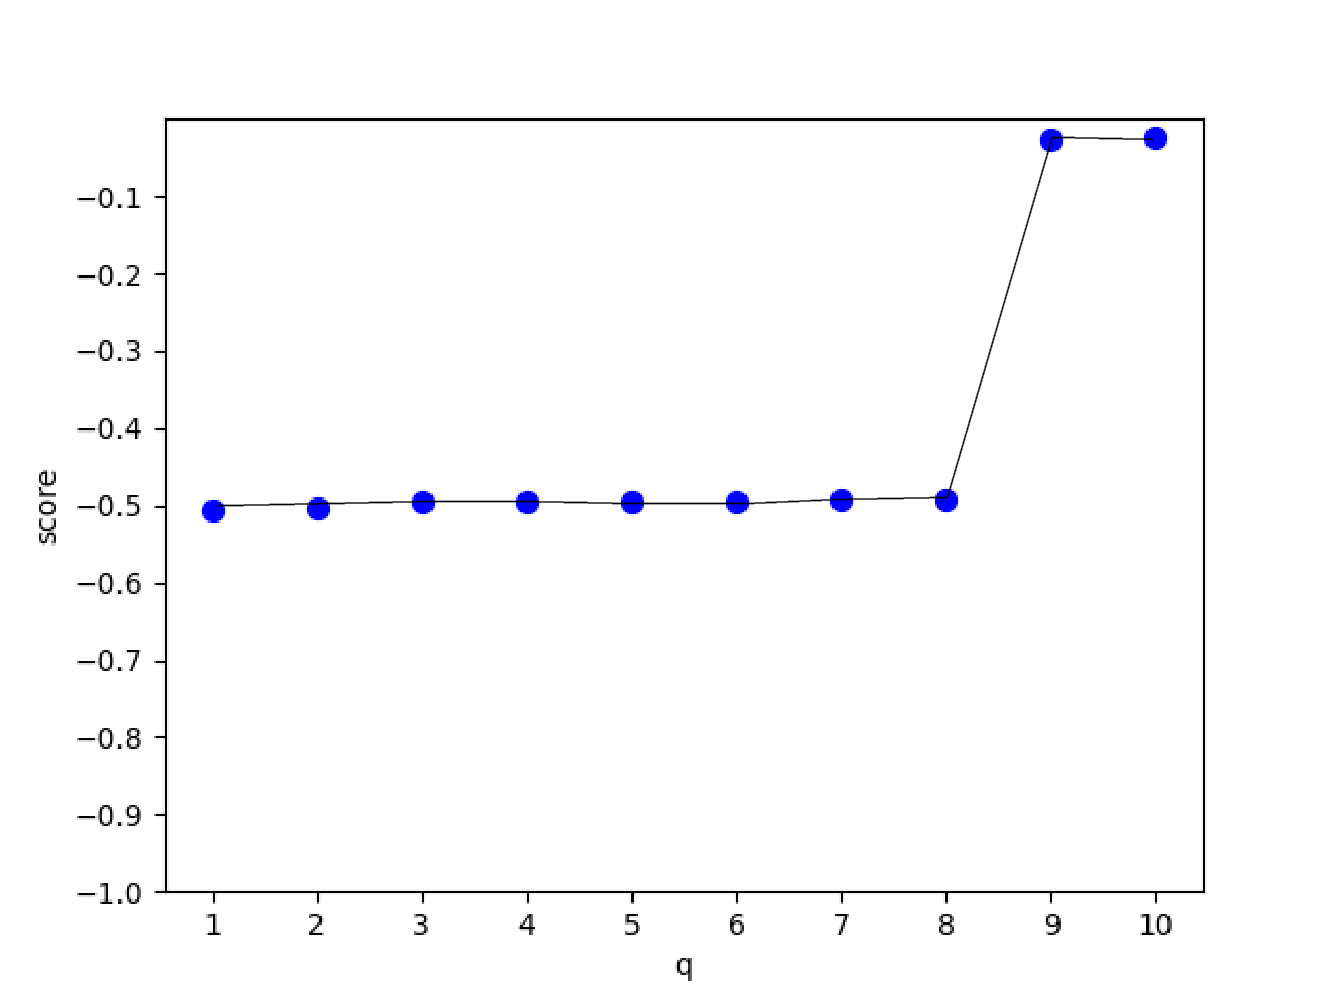
\includegraphics[width=0.6\textwidth]{问题五score.png}
     \caption{遗传算法误差$\mathrm{RMSE}$与$q$值的关系}
     \label{fig:遗传算法误差与q值的关系}
   \end{figure}
   由图可知,在$q$值小于8之前,最优估计对应 的误差都基本保持不变,当$q$超过8之后,$\mathcal{P}$将覆盖更大的离散空间,更有可能包含全局最优值在内,因此完成可以使最优估计对应 的适应度得分增加,这与预想 是一致的,即增加矩阵元素的位数可以提高精度。
   \begin{figure}[H]
     \centering
     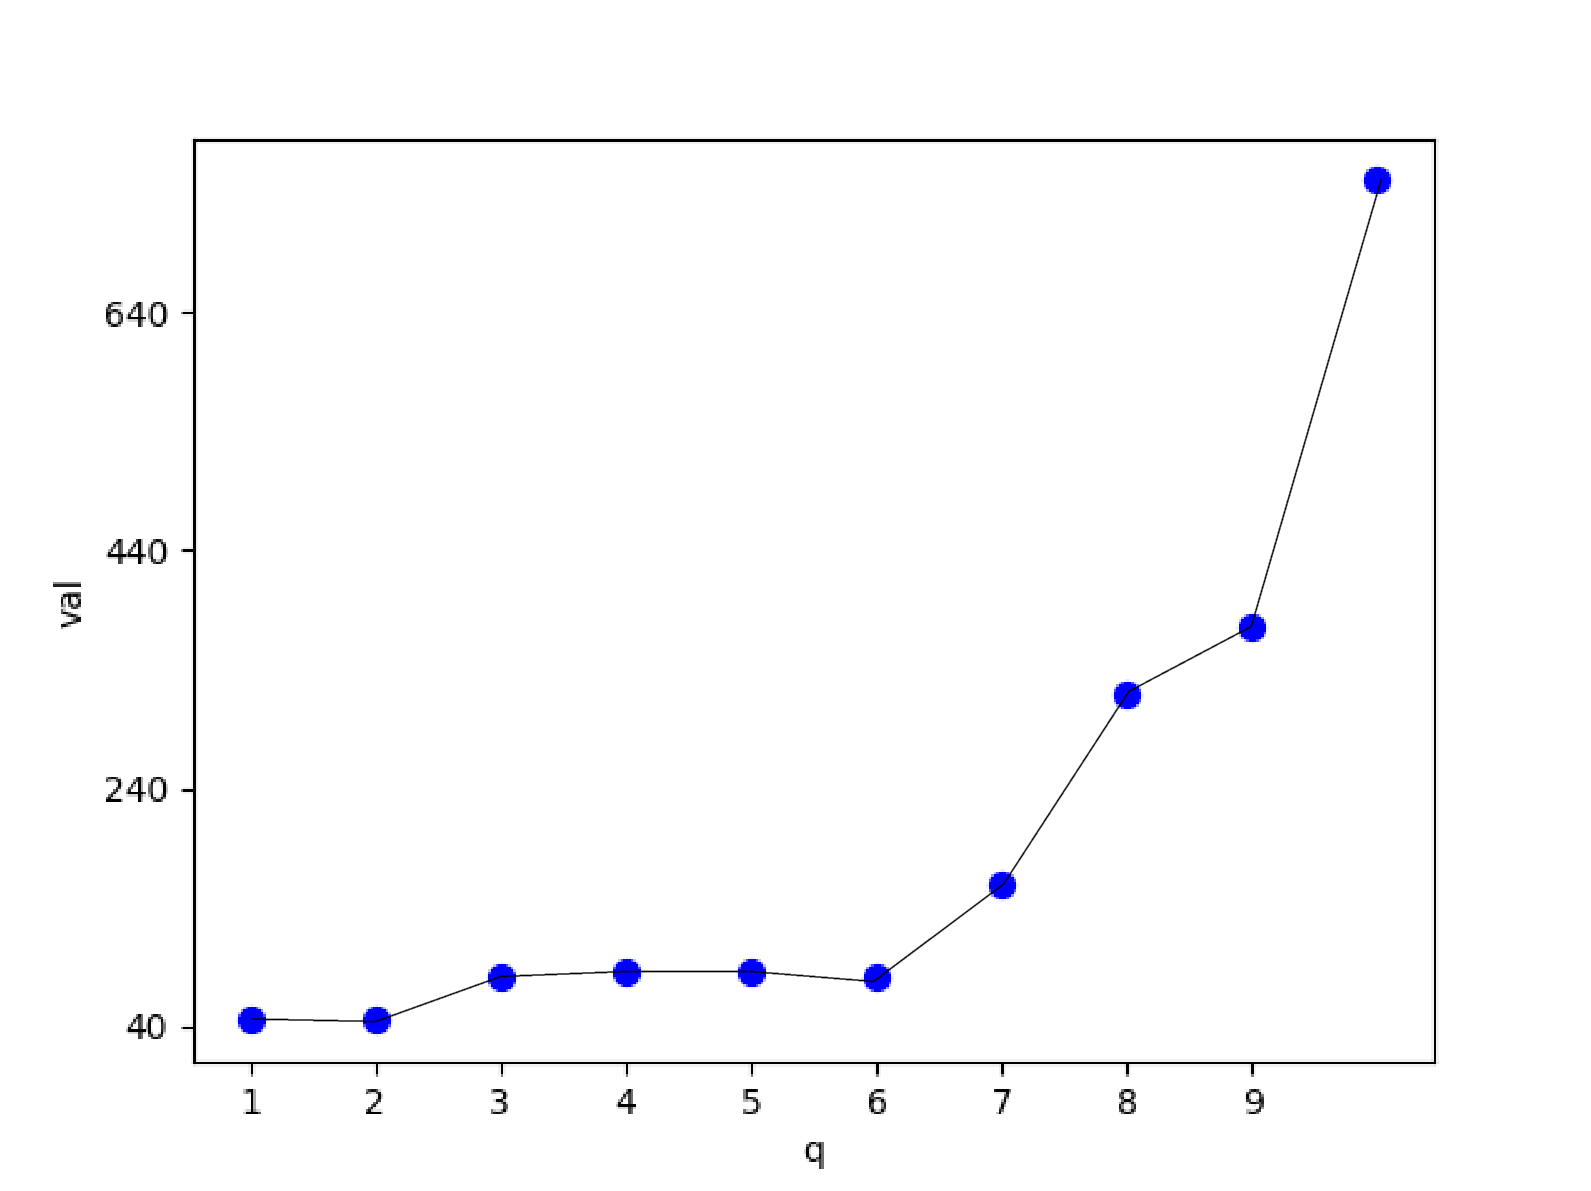
\includegraphics[width=0.6\textwidth]{问题五val.png}
     \caption{量化参数$\alpha$与$q$值的关系}
     \label{fig:量化参数与q值的关系}
   \end{figure}
 \end{subsection}
 图\ref{fig:量化参数与q值的关系}反映了随着$q$值的增加,量化参数$\alpha$也随之增加,这说明位数增加使得量化取值区间更为精细,因此量化效果将提升,与图\ref{fig:量化参数与q值的关系}反映的基本事实是一致的。
\end{section}

\begin{section}{结论}
 本文基于连续矩阵空间的可导性,使用正则项修正的梯度下降算法递推求解局部最小值,可分性。总的来说,对于给定已知的N维DFT矩阵$\mathbf{F}_N$,针对不同约束条件,我们均可以做到设计K个矩阵$\mathcal{A}=\{\mathbf{A}_1,\mathbf{A}_2,\cdots,\mathbf{A}_K\}$,使得矩阵$β\mathbf{F}_N$ 和$\mathbf{A}_1, \mathbf{A}_2,\cdots,\mathbf{A}_K$在Frobenius范数意义下尽可能接近,也即用一连串稀疏的、元素取值有限的矩阵连乘形式来近似表达DFT矩阵。
 对于问题一:在满足约束1的条件下,我们通过正则项修正后的梯度下降算法,生成了每行至多只有2个非零元素的稀疏矩阵,通过参数的选择,使得最优化问题得以解决。在DFT矩阵$\mathbf{F}_N$取$N=2^t,t=1,2,3,4,5$时,我们都能找到这样的稀疏矩阵去模拟DFT矩阵$\mathbf{F}_N$。通过绘制实验图像,证明了在我们的算法下有最小误差以及硬件复杂度。
 对于问题二:请在满足约束2的条件下,我们在梯度下降算法求出连续空间局部最优解的基础上,使用带约束的遗传算法进一步逼近真值,生成了元素取值优先的矩阵,其实部和虚部属于集合$P={0,\pm1,\pm2,\cdots,\pm2^{q-1} }$。通过参数的选择,使得最优化问题得以解决。在的DFT矩阵$\mathbf{F}_N$取$N=2^t,t=1,2,3,4,5$,我们都能找到这样的稀疏矩阵去模拟DFT矩阵$\mathbf{F}_N$。通过绘制实验图像,证明了在我们的算法下有最小误差以及硬件复杂度。
 对于问题三:我们通过将问题一和问题二的算法结合,同时限制了拟合矩阵的稀疏性和取值范围,用过参数的选择,使得最优化问题得以解决。在的DFT矩阵$\mathbf{F}_N$取$N=2^t,t=1,2,3,4,5$,我们都能找到这样的稀疏矩阵去模拟DFT矩阵$\mathbf{F}_N$。通过绘制实验图像,证明了在我们的算法下有最小误差以及硬件复杂度。
 对于问题五, 由于考虑了精度限制,我们对问题三的算法进行了改进,通过参数的选择,使得最优化问题得以解决。在的DFT矩阵$\mathbf{F}_N$取$N=2^t,t=1,2,3,4,5$,我们都能找到这样的稀疏矩阵去模拟DFT矩阵$\mathbf{F}_N$。通过绘制实验图像,证明了在我们的算法下有最小误差以及硬件复杂度。
\end{section}
\newpage
\printbibliography[heading=bibliography,title=\centering 参考文献]
\newpage
\begin{section}{附录·矩阵分解结果}
 本部分用于陈列各个题目分解得到的矩阵序列、计算函数以及Frobenius范数意义下的均方根误差。部分算式附于下:
 从分解矩阵序列中计算近似DFT矩阵的算式为:
 \begin{align*}
   \mathbf{F}_N\approx\frac{1}{\beta\alpha^K}\cdot\mathbf{A}_1\mathbf{A}_2\cdots\mathbf{A}_K
 \end{align*}
 其中,$\alpha$是量化参数,$\beta$是倍缩因子,$K$是分解得到的矩阵个数,$N$是矩阵的阶数,$\mathbf{A}_i$是分解得到的矩阵序列中的第$i$个矩阵。\par
 近似误差定义为:
 \begin{align*}
   \mathrm{RMSE}(\mathcal{A},\beta)=\frac{1}{N}\sqrt{||\beta\mathbf{F}_N-\mathbf{A_1A_2\cdots A}_K||_F^2}
 \end{align*}
 列出的表格将包含倍缩因子、量化参数和近似误差。
 \begin{center}
   $\beta=0.8418,\mathrm{RMSE}=0.000227,C=4$情况下的分解结果$N=1,K=1$
   \begin{align*}
     \mathbf{A}_1=
     \left[
       \begin{matrix}
         0.85305 & 0.8529                        \\
         0.8534  & -0.8503+2.153\times 10^{-15}j
       \end{matrix}
       \right]
   \end{align*}
 \end{center}

 \begin{center}
   $\beta=0.1422,\mathrm{RMSE}=0.4443,C=22$情况下的分解结果$N=4,K=2$
   \begin{align*}
     \mathbf{A}_1=\left[
       \begin{matrix}
         0            & 0.712+0.225j  & 0             & 0.549-0.207j \\
         0            & 0.212+0.339j  & -0.366-0.060j & 0            \\
         0            & -0.060+0.375j & 0             & 0.037-0.297j \\
         0.495+0.109j & 0.217+0.363j  & 0             & 0            \\
       \end{matrix}
       \right]
   \end{align*}\\
   \begin{align*}
     \mathbf{A}_2=\left[
       \begin{matrix}
         0.845+0.168j & 0            & -0.583-0.028j & 0 \\
         0.751+0.143j & 0            & 0.583-0.050j  & 0 \\
         0.806+0.124j & 0.436+0.084j & 0             & 0 \\
         0.766+0.066j & 0            & 0.397-0.061j  & 0 \\
       \end{matrix}
       \right]
   \end{align*}
 \end{center}


 \begin{center}
   $\beta=0.096,\mathrm{RMSE}=0.106,C=38$情况下的分解结果$N=4,K=3$
   \begin{align*}
     \mathbf{A}_1 & =\left[
       \begin{matrix}
         0             & 0.599-0.019j & 0            & 0.483+0.082j \\
         0             & 0.277+0.276j & 0.535-0.079j & 0            \\
         0             & 0.599+0.057j & 0.544-0.003j & 0            \\
         -0.174-0.053j & 0.061+0.154j & 0            & 0            \\
       \end{matrix}
     \right]                \\
     \mathbf{A}_2 & =\left[
       \begin{matrix}
         0            & 0            & 0.938+0.005j & 0.360+0.003j  \\
         0.499-0.090j & 0            & 0            & -0.495-0.200j \\
         0            & 0.343+0.009j & 0            & 0.376-0.038j  \\
         0.443-0.049j & 0            & 0            & 0.514-0.175j  \\
       \end{matrix}
     \right]                \\
     \mathbf{A}_3 & =\left[
       \begin{matrix}
         0            & -0.216+0.235j & 0            & -0.029-0.190j \\
         0.558-0.045j & 0.485+0.220j  & 0            & 0             \\
         0.379-0.069j & -0.106+0.302j & 0            & 0             \\
         0            & 0             & 0.600+0.055j & 0.538-0.018j  \\
       \end{matrix}
       \right]
   \end{align*}
 \end{center}

\end{section}

\begin{section}{附录·解决方案代码}
 代码的文件夹层级与相应功能解释对应如下:
 \begin{figure}[H]
   \centering
   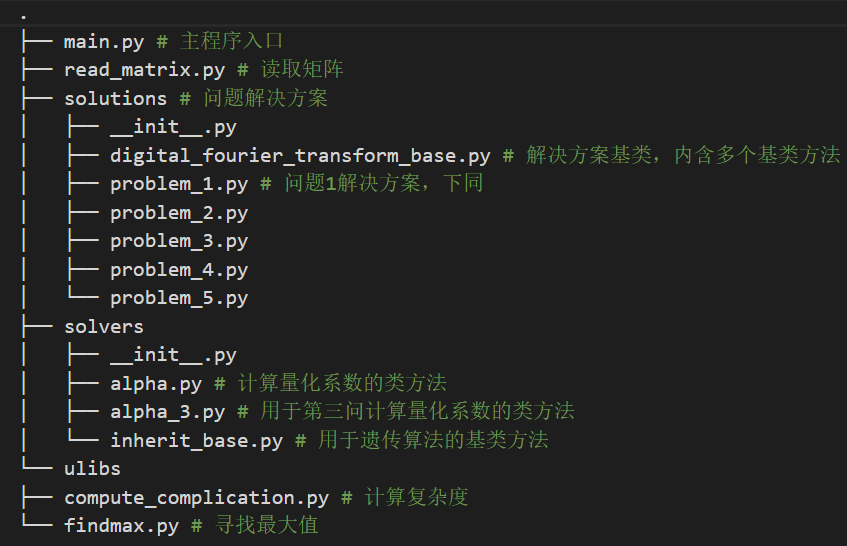
\includegraphics[width=0.8\textwidth]{代码文件层级.png}
   \caption{代码文件层级}
   \label{fig:代码文件层级}
 \end{figure}
 梯度下降法核心基类代码实现如下:
 \begin{lstlisting}[language=Python ]
  import numpy as np
  import itertools
  from typing import List, Iterable
  
  
  class DigitalFourierTransformerBase:
      def __init__(self, N: int, K: int, **kwargs) -> None:
          self.K = K
          self.N = N
          self._dft = np.zeros([N, N], dtype=complex)
          self._A_K = [np.random.random([N, N]).astype(complex)
                       for i in range(K)]
          self.beta = 1
  
      @property
      def get_beta(self):
          return self.beta
  
      @staticmethod
      def frobenius(A: np.ndarray) -> float:
          return np.sum(np.square(np.abs(A)))
  
      @property
      def A_K(self):
          return self._A_K
  
      @property
      def dft(self):
          for i in range(self.N):
              for j in range(self.N):
                  self._dft[i, j] = np.exp(-2j * np.pi * i * j / self.N)
          return self._dft
  
      @property
      def result(self):
          """
          输出最终的连乘积拟合结果
          """
          return self._matmul(self._A_K, self.K)
  
      def _matmul(self, A: List[np.ndarray], k: int):
          """
          矩阵连乘积,排除了第k个元素的顺序乘
          """
          try:
              temp = np.identity(self.N)
              for i in range(k):
                  temp = temp @ A[i]
              for i in range(k + 1, self.K):
                  temp = A[i] @ temp
              return temp
          except Exception as exc:
              print("here!")
              print(exc)
              return np.nan
  
      @property
      def error(self):
          return DigitalFourierTransformerBase.frobenius(
              np.abs(self.beta * self.dft - self._matmul(self._A_K, self.K))
          )/self.N
  
      def print(self, **kwargs):
          print(f"beta:{self.beta}")
          for i in range(self.K):
              print(f"A_{i}:\n{self._A_K[i]}")
          print(f"result:{self.result}")
          print(f"complex_degree:{self.comlexity}")
  
      def train(self, lr: float = 0.01, epoch: int = 1000, is_post_train: bool = False, **kwargs):
          raise NotImplementedError
  
      def post_train(self, store_path: str, **kwargs):
          raise NotImplementedError
  
      def grad(self, k: int, **kwargs):
          raise NotImplementedError
  
      def grad_beta(self):
          raise NotImplementedError
  
      def max_two(self, A_k: np.ndarray) -> np.ndarray:
          """
          找到最大和第二大的行元素
          """
  
          def _max_row(A: np.ndarray):
              assert A.shape.__len__() == 2
              array_blank = np.zeros_like(A)
              array_blank[range(A.shape[1]), np.argmax(np.abs(A), axis=1)] = A[
                  range(A.shape[1]), np.argmax(np.abs(A), axis=1)
              ]
              return array_blank
  
          max_1_mat = _max_row(A_k)
          max_2_mat = _max_row(A_k - max_1_mat)
          return max_1_mat + max_2_mat
  
      @property
      def comlexity(self):
          def _compute_complex(A1, A2) -> int:
              def _compare_float(a, b):
                  if abs(a - b) <= 1e-4:
                      return 1
                  return 0
  
              def judge_complex(c):
                  index = [0, 1, -1]
                  _sum = sum(
                      itertools.starmap(
                          lambda x, y: _compare_float(c.real, x)
                          * _compare_float(c.imag, y),
                          itertools.product(index, index),
                      )
                  )
                  return 1 - _sum
  
              complex_degree = 0
              # for i in range(len(A1)):  # A1矩阵的行
              complex_degree = sum(
                  map(
                      lambda A1_i: sum(
                          map(
                              lambda j: sum(
                                  itertools.starmap(
                                      lambda x, y: judge_complex(
                                          x) * judge_complex(y[j]),
                                      zip(A1_i, A2),
                                  )
                              ),
                              range(len(A2)),
                          )
                      ),
                      A1,
                  )
              )
              return complex_degree
  
          temp = self._A_K[0]
          complex_degree = 0
          for A_K_i in self._A_K[1:]:
              complex_degree += _compute_complex(temp, A_K_i)
              temp = temp @ A_K_i
          return complex_degree
  
  \end{lstlisting}
 遗传算法核心基类代码:
 \begin{lstlisting}[language=Python]
    import itertools
  from typing import Any, Callable, List, Tuple, Union, Iterable
  
  
  class InheritSolverBase:
      def __init__(self, individual_num: int, individual: Callable, **kwargs) -> None:
          """
          Arguments:
           - `individual_num`: 个体数量
           - `individual`: 个体类的构造函数
           - `kwargs`: 个体类的构造函数的参数
          """
          self.group = [individual(**kwargs) for i in range(individual_num)]
  
      def _filter(self, **kwargs):
          """
          Arguments:
           - `group`: 种群
           - `filter`: 与环境相关的过滤函数,返回值为bool
          """
          raise NotImplementedError
  
      def _multiply(self, individual: object, **kwargs) -> object:
          """
          Arguments:
           - `group`: 种群
           - `multiply`: 与环境相关的繁殖函数,返回值为新的个体
          """
          raise NotImplementedError
  
      def _survive(self, **kwargs) -> None:
          """
          自然死亡的
          """
          raise NotImplementedError
  
      def train(
          self,
          epoch_num: int = 100,
          survive_kwargs: dict = {},
          multiply_kwargs: dict = {},
          filter_kwargs: dict = {},
      ) -> List[object]:
          score = -10000000000
          score_new = 0
          for i in range(epoch_num):
              if i != 0:
                  self._survive(**survive_kwargs)
              # 进行一次繁殖,这个函数里面应该包含了变异和自然死亡
              temp_group = list(
                  map(
                      lambda x: list(self._multiply(x, **multiply_kwargs)),
                      self.group,
                  )
              )
              self.group = list(itertools.chain(*temp_group))
              if i % 5 == 0:
                  # 进行一次过滤
                  score_new = self._filter(**filter_kwargs)
                  if abs(score_new - score) < 1e-10 and i % 100 == 0:
                      break
                  score = score_new
          return self.group  # 返回最后一代的种群
  
   \end{lstlisting}
 遗传算法核心实现代码如下:
 \begin{lstlisting}[language=Python]
    from solvers.inherit_base import InheritSolverBase
    from typing import Callable, List, Tuple, Union, Iterable
    import random
    import numpy as np
    
    
    class Individual:
        """
        每个个体都是一个服从正态分布的随机变量,出生的后代依概率出生
        """
    
        def __init__(self, val: float = 1, sigma: float = 0.2, age: int = 0) -> None:
            """
            Arguments:
             - `val`: 个体的值
             - `sigma`: 个体繁殖后代时的标准差
             - `age`: 个体的年龄,用于在过滤时判断个体是否应该死亡
            """
            self.val = val
            self.sigma = sigma
            self.age = age
            self._score = -np.inf
    
        def __call__(self, val: float = 1, sigma: float = 0.2) -> "Individual":
            return Individual(val, sigma)
    
        def _multiply(
            self, age_gate: int = 20, offstring_num: int = 8
        ) -> List["Individual"]:
            if random.random() > np.exp(age_gate - self.age):
                # 个体死亡
                return []
            else:
                self.age += 1
                return [
                    self,
                    *list(
                        Individual(abs(val), self.sigma)._change()
                        for val in np.random.normal(self.val, self.sigma, offstring_num)
                    ),
                ]
    
        def _change(
            self,
            gate: List[float] = [0.03, 0.03, 0.1, 0.1],
            rate: List[float] = [1.25, 1.25],
        ) -> object:
            """
            用于变异的函数,每个参数都有一定的概率变异,变异的方式是乘以一个确定的数
            """
            if random.random() < gate[0]:
                self.val *= rate[0]
            if random.random() < gate[1]:
                self.val /= rate[0]
            elif random.random() < gate[2]:
                self.sigma *= rate[1]
            elif random.random() < gate[3]:
                self.sigma /= rate[1]
            return self
    
        def score(
            self, dft: np.ndarray, A_K: List[np.ndarray], K: int, beta: float
        ) -> float:
            if self._score != -np.inf:
                return self._score
    
            def _quantify(A: np.ndarray):
                B = np.zeros_like(A, dtype=int)
                A_real = np.real(A)
                A_imag = np.imag(A)
                B = (
                    np.sign(A_real)
                    * 2 ** np.floor((np.clip(np.log2(np.abs(A_real)), 0, None)))
                    + np.sign(A_imag)
                    * 2 ** np.floor((np.clip(np.log2(np.abs(A_imag)), 0, None)))
                    * 1j
                )
                return B
    
            self._score = (
                -np.sqrt(
                    np.sum(
                        np.abs(
                            beta * dft
                            - self.matmul(
                                map(lambda x: _quantify(
                                    self.val * x) / self.val, A_K), K
                            )
                        )
                    )
                )
                / A_K[0].shape[0]
            )
            return self._score
    
        def matmul(self, A: Iterable[np.ndarray], k: int):
            i = 1
            for a in A:
                if i == 1:
                    temp = a
                    i += 1
                else:
                    temp = temp @ a
            return temp
    
    
    class AlphaInherit(InheritSolverBase):
        def __init__(
            self,
            individual_num: int,
            individual: Callable[..., Individual],
            dft: np.ndarray,
            A_K: List[np.ndarray],
            K: int,
            beta: float,
            gate: float,
            val: Iterable[float],
            sigma: Iterable[float],
            lr: float,
            **kwargs,
        ) -> None:
            self.dft = dft
            self.A_K = A_K
            self.K = K
            self.beta = beta
            self.gate = gate
            self.lr = lr
            self.group = [individual(v, s) for v, s in zip(val, sigma)]
    
        def _filter(
            self,
            gate: float = -500,
        ) -> float:
            gate = self.gate if self.gate else gate
            score = [
                (i, individual.score(self.dft, self.A_K, self.K, self.beta))
                for i, individual in enumerate(self.group)
            ]
            score = sorted(score, key=lambda x: x[1])
            # 淘汰小于gate的个体,如果都不小于gate,则淘汰后80%的个体
            # 如果都小于,则保留后20%的个体
            for i in range(len(score)):
                if score[i][1] > gate:
                    # if score[i][1] > gate and i > len(score) * 0.8:
                    self.group = [self.group[j] for j, s in score[i:]]
                    print(f"score: {score[-1][1]}")
                    self.gate = max(score[-1][1], self.gate + self.lr)
                    return score[-1][1]
            self.group = [self.group[j] for j, s in score[int(len(score) * 0.85):]]
            print(f"score: {score[-1][1]}")
            self.gate = max(score[-1][1], self.gate + self.lr)
            return score[-1][1]
    
        def _survive(
            self,
        ) -> object:
            score = [
                (i, individual.score(self.dft, self.A_K, self.K, self.beta))
                for i, individual in enumerate(self.group)
            ]
            score = sorted(score, key=lambda x: x[1])
            # 淘汰后80%的个体
            self.group = [self.group[i] for i, s in score[int(len(score) * 0.85):]]
    
        def _multiply(
            self, individual: Individual, age_gate: int = 20, **kwargs
        ) -> List[Individual]:
            return individual._multiply(age_gate=age_gate, **kwargs)
  \end{lstlisting}
 以下是问题一的解决方案代码,该代码从梯度下降基类继承而来:
 \begin{lstlisting}[language=Python]
    # 抽象的DFT矩阵分解基类
    import numpy as np
    from solutions.digital_fourier_transform_base import DigitalFourierTransformerBase
    import pickle
    import os
    
    
    class DFT_1(DigitalFourierTransformerBase):
        @property
        def __name__(self):
            return "Problem_1"
    
        def identify(self, A_k: np.ndarray, rate: float = 0.00001) -> np.ndarray:
            """
            使用一波最原始的方法,取出每行的绝对值最大的元素,将其放大某个倍数,然后将第二大的也放大这个位数,将其他的缩小某个倍数。
            """
            res = A_k - self.max_two(A_k)
            return res * (1 - rate) + self.max_two(A_k) * (1 + rate)
    
        def grad(self, k: int, m: float = 3):
            return (
                -(self.beta * self.dft - self._matmul(self._A_K, self.K))
                @ np.conjugate(self._matmul(self._A_K, k))
                - self._matmul(self._A_K, k)
                @ np.conjugate((self.beta * self.dft - self._matmul(self._A_K, self.K)))
                * m
            )
    
        def grad_beta(self):
            return np.real(
                np.trace(
                    (self.beta * self.dft - self._matmul(self._A_K, self.K))
                    @ np.conjugate(self.dft)
                )
            )
    
        def train(self, lr: float = 0.01, epoch: int = 1000, store_path: os.PathLike = './result', **kwargs):
            error = 100000
            error_list = []
            beta_list = []
            A_K_list = []
            for i in range(epoch):
                try:
                    A_K_temp = [
                        self.identify(x - lr * self.grad(k))
                        for k, x in enumerate(self._A_K)
                    ]
                    beta_temp = self.beta - lr * self.grad_beta()
                    if np.abs(self.error - error) < 1e-8:
                        break
    
                    if i % 100 == 0:
                        # error = self.error
                        print(f"epoch:{i}, error:{self.error}")
                    error = self.error
                    self._A_K = A_K_temp
                    self.beta = beta_temp
                    error_list.append(error)
                    A_K_list.append(A_K_temp)
                    beta_list.append(beta_temp)
                except:
                    raise Exception("TrainError")
            self._A_K = [self.max_two(A_K_i) for A_K_i in self._A_K]
            pickle.dump((self, error_list, A_K_list, beta_list),
                        open(os.path.join(store_path, f"K{self.K}_N{self.N}_lr{lr}_"+self.__name__+'.pkl'), 'wb'))    
 \end{lstlisting}
 以下是问题二的解决方案代码,该代码也从梯度下降基类继承而来,使用了遗传算法作为对象处理后续:
 \begin{lstlisting}[language=Python]
  # 抽象的DFT矩阵分解基类
import numpy as np
from solutions.digital_fourier_transform_base import DigitalFourierTransformerBase
from solvers.alpha import Individual, AlphaInherit
import pickle
import os


class DFT_2(DigitalFourierTransformerBase):
    @property
    def __name__(self):
        return "Problem_2"

    def identify(self, A_k: np.ndarray, rate: float = 0.00001) -> np.ndarray:
        """
        使用一波最原始的方法,取出每行的绝对值最大的元素,将其放大某个倍数,然后将第二大的也放大这个位数,将其他的缩小某个倍数。
        """
        res = A_k - self.max_two(A_k)
        return res * (1 - rate) + self.max_two(A_k) * (1 + rate)

    def grad(self, k: int, m: float = 3):
        return (
            -(self.beta * self.dft - self._matmul(self._A_K, self.K))
            @ np.conjugate(self._matmul(self._A_K, k))
            - self._matmul(self._A_K, k)
            @ np.conjugate((self.beta * self.dft - self._matmul(self._A_K, self.K)))
            * m
        )

    def grad_beta(self):
        return np.real(
            np.trace(
                (self.beta * self.dft - self._matmul(self._A_K, self.K))
                @ np.conjugate(self.dft)
            )
        )

    def train(
        self, lr: float = 0.01, epoch: int = 1000, store_path="./result/Problem_2.pkl", is_post_train: bool = False, **kwargs
    ):
        error_list = []
        A_K_list = []
        beta_list = []
        self.lr = lr
        error = 100000
        for i in range(epoch):
            try:
                A_K_temp = [x - lr * self.grad(k)
                            for k, x in enumerate(self._A_K)]
                beta_temp = self.beta - lr * self.grad_beta()
                if self.error - error > 0:
                    break
                if i % 100 == 0:
                    # error = self.error
                    print(f"epoch:{i}, error:{self.error}")
                error = self.error
                self._A_K = A_K_temp
                self.beta = beta_temp
                error_list.append(self.error)
                A_K_list.append(self._A_K)
                beta_list.append(self.beta)
            except:
                raise Exception("TrainError")
        pickle.dump((self, error_list, A_K_list, beta_list), open(os.path.join(
                    store_path, f"K{self.K}_N{self.N}_lr{lr}_"+self.__name__+".pkl"), "wb"))
        if is_post_train:
            self.post_train(store_path=store_path, **kwargs)

    def convert_to_power_of_two(self, A: np.ndarray):
        B = np.zeros_like(A, dtype=int)
        A_real = np.real(A)
        A_imag = np.imag(A)
        B = (
            np.sign(A_real)
            * 2 ** np.floor((np.clip(np.log2(np.abs(A_real)), 0, None)))
            + np.sign(A_imag)
            * 2 ** np.floor((np.clip(np.log2(np.abs(A_imag)), 0, None)))
            * 1j
        )
        return B

    def post_train(
        self,
        store_path: str = "./result/Problem_2.pkl",
        iter_num: int = 10000,
        individual_num: int = 8,
        offstring_num: int = 8,
    ):
        """
        后期操作,在完成浮点训练之后,进行一次规划,由于规划的目标函数不可以求导,不能使用梯度下降,替代梯度的方法也不好做,这里尝试使用智能优化算法遗传算法来做。
        """
        print("*"*50)
        print("现在进入遗传算法内")
        print("*"*50)
        M, _, _, _ = pickle.load(
            open(os.path.join(store_path, f"K{self.K}_N{self.N}_lr{self.lr}_"+self.__name__+".pkl"), "rb"))
        IS = AlphaInherit(
            individual_num,
            Individual,
            val=np.random.normal(2, 1, individual_num),
            sigma=np.random.normal(0.4, 0.1, individual_num),
            dft=M.dft,
            beta=M.get_beta,
            A_K=M.A_K,
            K=M.K,
            gate=-30,
            lr=1e-4
        )
        final_group = IS.train(
            epoch_num=iter_num,
            multiply_kwargs={"offstring_num": offstring_num},
            filter_kwargs={},
        )
        val = 0
        min_obj = None
        for i in final_group:
            if val > i.score(M.dft, M.A_K, M.K, M.get_beta):
                val = i.score(M.dft, M.A_K, M.K, M.get_beta)
                min_obj = i

        self._A_K = [self.convert_to_power_of_two(
            min_obj.val*A_K_i) for A_K_i in M._A_K]
        self.alpha = min_obj.val
        print(
            f"拟合结果与真实值的差: {val}, 拟合因子: {min_obj.val}, 拟合因子的标准差: {min_obj.sigma}")
        pickle.dump(
            (self, min_obj),
            open(os.path.join(store_path, self.__name__ +
                 "_processed" + ".pkl"), "wb"),
        )

    @property
    def result(self):
        """
        输出最终的连乘积拟合结果
        """
        return self._matmul(self._A_K / self.alpha, self.K)

    def print(self, **kwargs):
        print(f"beta:{self.beta}")
        for i in range(self.K):
            print(f"A_{i}:\n{self._A_K[i]}")
        print(f"result:{self.result}")
        print(f"complex_degree:{self.comlexity}")
        self._A_K = [A_K_i/self.alpha for A_K_i in self._A_K]
        print(f"error:{self.error/self.N}")

 \end{lstlisting}
 问题三解决方案,由于问题三由问题二引申而来,因此本方案继承自问题二的类:
 \begin{lstlisting}[language=Python]
  # 抽象的DFT矩阵分解基类
import pickle
import numpy as np
from solutions.problem_2 import DFT_2
import os
from solvers import Individual_3, AlphaInherit


class DFT_3(DFT_2):
    @property
    def __name__(self):
        return "Problem_3"

    def train(
        self, lr: float = 0.01, epoch: int = 1000, store_path="./result/Problem_3.pkl", is_post_train: bool = False, **kwargs
    ):
        error = 100000
        error_list = []
        A_K_list = []
        beta_list = []
        self.lr=lr
        for i in range(epoch):
            try:
                A_K_temp = [
                    self.identify(x - lr * self.grad(k))
                    for k, x in enumerate(self._A_K)
                ]
                beta_temp = self.beta - lr * self.grad_beta()
                if self.error - error > 0:
                    break
                if i % 100 == 0:
                    # error = self.error
                    print(f"epoch:{i}, error:{self.error}")
                error = self.error
                self._A_K = A_K_temp
                self.beta = beta_temp
                error_list.append(self.error)
                A_K_list.append(self._A_K)
                beta_list.append(self.beta)
            except:
                raise Exception("Here! Error!")
        pickle.dump((self, error_list, A_K_list, beta_list), open(os.path.join(
                    store_path, f"K{self.K}_N{self.N}_lr{lr}_"+self.__name__+".pkl"), "wb"))
        if is_post_train:
            self.post_train(store_path=store_path, **kwargs)

    def post_train(
        self,
        store_path: str = "./result/Problem_3.pkl",
        iter_num: int = 10000,
        individual_num: int = 8,
        offstring_num: int = 8,
    ):
        """
        后期操作,在完成浮点训练之后,进行一次规划,由于规划的目标函数不可以求导,不能使用梯度下降,替代梯度的方法也不好做,这里尝试使用智能优化算法遗传算法来做。
        """
        print("*"*50)
        print("现在进入遗传算法内")
        print("*"*50)
        M, _, _, _ = pickle.load(
            open(os.path.join(store_path, f"K{self.K}_N{self.N}_lr{self.lr}_"+self.__name__+".pkl"), "rb"))
        IS = AlphaInherit(
            individual_num,
            Individual_3,
            val=np.random.normal(35000, 400, individual_num),
            sigma=np.random.normal(8000, 200, individual_num),
            dft=M.dft,
            beta=M.get_beta,
            A_K=M.A_K,
            K=M.K,
            gate=-30,
            lr=1e-4
        )
        final_group = IS.train(
            epoch_num=iter_num,
            multiply_kwargs={"offstring_num": offstring_num},
            filter_kwargs={},
        )
        val = 0
        min_obj = None
        for i in final_group:
            if val > i.score(M.dft, M.A_K, M.K, M.get_beta):
                val = i.score(M.dft, M.A_K, M.K, M.get_beta)
                min_obj = i

        self._A_K = [self.convert_to_power_of_two(
            self.max_two(min_obj.val*A_K_i)) for A_K_i in M._A_K]
        self.alpha = min_obj.val
        print(
            f"拟合结果与真实值的差: {val}, 拟合因子: {min_obj.val}, 拟合因子的标准差: {min_obj.sigma}")
        pickle.dump(
            (self, min_obj),
            open(os.path.join(store_path, self.__name__ +
                 "_processed" + ".pkl"), "wb"),
        )

 \end{lstlisting}
 问题四没有提供解决方案代码,因为问题四可以由问题二和问题三实现,以下是问题五的解决方案代码,该代码同样继承着问题二,同时使用了遗传算法作为对象处理后续:
 \begin{lstlisting}[language=Python]
  # 抽象的DFT矩阵分解基类
import pickle
import numpy as np
from solutions.problem_2 import DFT_2
import os
from solvers import Individual_3, AlphaInherit


class DFT_5(DFT_2):
    @property
    def __name__(self):
        return "Problem_5"

    def train(
        self, lr: float = 0.01, epoch: int = 1000, store_path="./result/Problem_5.pkl", is_post_train: bool = False, **kwargs
    ):
        error = 100000
        error_list = []
        A_K_list = []
        beta_list = []
        self.lr = lr
        for i in range(epoch):
            try:
                A_K_temp = [
                    self.identify(x - lr * self.grad(k))
                    for k, x in enumerate(self._A_K)
                ]
                beta_temp = self.beta - lr * self.grad_beta()
                if self.error - error > 0:
                    break
                if i % 100 == 0:
                    print(f"epoch:{i}, error:{self.error}")
                error = self.error
                self._A_K = A_K_temp
                self.beta = beta_temp
                error_list.append(self.error)
                A_K_list.append(self._A_K)
                beta_list.append(self.beta)
            except:
                raise Exception("Here! Error!")
        pickle.dump((self, error_list, A_K_list, beta_list), open(os.path.join(
                    store_path, f"K{self.K}_N{self.N}_lr{lr}_"+self.__name__+".pkl"), "wb"))
        if is_post_train:
            self.post_train(store_path=store_path, **kwargs)

    def post_train(
        self,
        store_path: str = "./result/Problem_3.pkl",
        iter_num: int = 10000,
        individual_num: int = 8,
        offstring_num: int = 8,
    ):
        """
        后期操作,在完成浮点训练之后,进行一次规划,由于规划的目标函数不可以求导,不能使用梯度下降,替代梯度的方法也不好做,这里尝试使用智能优化算法遗传算法来做。
        """
        print("*"*50)
        print("现在进入遗传算法内")
        print("*"*50)
        if not os.path.exists(os.path.join(store_path, 'problem_5')):
            os.mkdir(os.path.join(store_path, 'problem_5'))
        for q in range(1, 17):
            print(f"此时是q={q}的遗传算法")
            print("*"*50)
            M, _, _, _ = pickle.load(
                open(os.path.join(store_path, f"K{self.K}_N{self.N}_lr{self.lr}_"+self.__name__+".pkl"), "rb"))
            IS = AlphaInherit(
                individual_num,
                Individual_3,
                val=np.random.normal(2**q, 0.5, individual_num),
                sigma=np.random.normal(0.4, 0.02, individual_num),
                dft=M.dft,
                beta=M.get_beta,
                A_K=M.A_K,
                K=M.K,
                gate=-30,
                lr=1e-4
            )
            final_group = IS.train(
                epoch_num=iter_num,
                multiply_kwargs={"offstring_num": offstring_num},
                filter_kwargs={},
            )
            val = 0
            min_obj = None
            for i in final_group:
                if val > i.score(M.dft, M.A_K, M.K, M.get_beta):
                    val = i.score(M.dft, M.A_K, M.K, M.get_beta)
                    min_obj = i

            self._A_K = [self.convert_to_power_of_two(
                self.max_two(min_obj.val*A_K_i)) for A_K_i in M._A_K]
            self.alpha = min_obj.val
            print(
                f"拟合结果与真实值的差: {val}, 拟合因子: {min_obj.val}, 拟合因子的标准差: {min_obj.sigma}")
            pickle.dump(
                (self, min_obj),
                open(os.path.join(store_path, 'problem_5', f"q{q}"+self.__name__ +
                                  "_processed" + ".pkl"), "wb"),
            )

 \end{lstlisting}
 用于问题三的特化遗传算法的实现代码如下:
 \begin{lstlisting}[language=Python]
  from solvers.alpha import Individual
import numpy as np
from typing import List


class Individual_3(Individual):
    def max_two(self, A_k: np.ndarray) -> np.ndarray:
        """
        找到最大和第二大的行元素
        """

        def _max_row(A: np.ndarray):
            assert A.shape.__len__() == 2
            array_blank = np.zeros_like(A)
            array_blank[range(A.shape[1]), np.argmax(np.abs(A), axis=1)] = A[
                range(A.shape[1]), np.argmax(np.abs(A), axis=1)
            ]
            return array_blank

        max_1_mat = _max_row(A_k)
        max_2_mat = _max_row(A_k - max_1_mat)
        return max_1_mat + max_2_mat

    def __call__(self, val: float = 1, sigma: float = 0.2) -> Individual:
        return Individual_3(val, sigma)

    def score(
        self, dft: np.ndarray, A_K: List[np.ndarray], K: int, beta: float
    ) -> float:
        if self._score != -np.inf:
            return self._score

        def _quantify(A: np.ndarray):
            B = np.zeros_like(A, dtype=int)
            A_real = np.real(A)
            A_imag = np.imag(A)
            B = (
                np.sign(A_real)
                * 2 ** np.ceil((np.clip(np.log2(np.abs(A_real)), 0, None)) - 1)
                + np.sign(A_imag)
                * 2 ** np.ceil((np.clip(np.log2(np.abs(A_imag)), 0, None)) - 1)
                * 1j
            )
            return B

        self._score = (
            -np.sqrt(
                np.sum(
                    np.abs(
                        beta * dft
                        - self.matmul(
                            map(lambda x: self.max_two(_quantify(
                                self.val * x)) / self.val, A_K), K
                        )
                    )
                )
            )
            / A_K[0].shape[0]
        )
        return self._score

 \end{lstlisting}
 最后,是主函数部分,调用以上各包并使用命令行解释器进行参数输入:
 \begin{lstlisting}[language=Python]
  from solutions import solver_1, solver_2, solver_3, solver_4, solver_5
import numpy as np
import os
import argparse


def parse():
    parser = argparse.ArgumentParser()
    parser.add_argument('--solver', type=int, default=1,
                        help='选择不同问题的解决方案,用整数表示,1-5')
    parser.add_argument('--lr', type=float, default=1e-6, help='学习率')
    parser.add_argument('--epoch', type=int, default=40000)
    parser.add_argument('--store_path', type=str,
                        default='./result', help='存储路径')
    parser.add_argument('--is_post_train', type=bool,
                        default=True, help='是否进行后期训练,即使用遗传算法进一步逼近')
    parser.add_argument('--rank', '-t', type=int,
                        default=2, help='矩阵的阶数,这里用的是2的t次方')
    parser.add_argument('--K', type=int, default=2, help='矩阵序列的个数')
    return parser.parse_args()


if __name__ == '__main__':
    args = parse()
    solvers = [solver_1, solver_2, solver_3, solver_4, solver_5]
    M = solvers[args.solver-1](2**args.rank, args.K)
    if not os.path.exists(args.store_path):
        os.mkdir(args.store_path)
    if args.solver == 1:
        args.is_post_train = False
    M.train(lr=args.lr, epoch=args.epoch, store_path=args.store_path,
            is_post_train=args.is_post_train)
    X = np.random.random([2**args.rank, 1]).astype(complex)
    print(M.beta * M.dft - M.result)
    M.print()

 \end{lstlisting}
\end{section}
\end{document}